

\section{Методы управления соединениями}

\subsection{Описание алгоритмов}

\subsubsection{Алгоритм с безусловным подтверждением}

 Для открытия соединения с соседней станцией станция отправляет служебный кадр Peering Open Frame, а также отвечает на полученный от соседней станции такой же кадр кадром Peering Confirm Frame. Для закрытия соединения станция отправляет станции, с которой соединение открыто, служебный кадр Peering Close Frame. Доставка всех служебных кадров подтверждается, и кадры, на которые не получено подтверждение, повторяются. Поэтому служебные кадры доставляются с вероятностью, близкой к единице, и состояние соединения с высокой вероятностью на обеих станциях оказывается синхронизованным. %, т.е. обе станции оценивают состояние соединения одинаково.

\begin{enumerate}
 \item Станция принимает решение об открытии соединения с соседней станцией, получив от нее подряд $r$ биконов.
 \item Станция принимает решение о закрытии существующего соединения, если не получила от станции, с которой открыто соединение, подряд $s$ биконов.%\footnote{Заметим, что решение о закрытии соединения может быть принято еще в одном случае, а именно, если по данному соединению не получается передать подряд определенное число пакетов данных.}
 \item Получив кадр Peering Open Frame или Peering Close Frame от соседней станции, станция всегда и без дополнительных проверок качества соединения, т.е. \emph{безусловно}, соглашается на соответственно открытие или закрытии соединения.
\end{enumerate}

 В статье параметры по умолчанию $r=1, s=5$. 
 
\subsubsection{Алгоритм с условным подтверждением}

Изменим третье правило алгоритма с безусловным подтверждением следующим образом: станция $A$, получив от соседней станции $B$ предложение об открытии соединения, соглашается на открытие только в том случае, если к моменту получения кадра Peering Open Frame станция $A$ получила от станции $B$ не менее $l$ биконов подряд. В противном случае станция $A$ отказывается от открытия соединения. Получив кадр Peering Close Frame от соседней станции, станция по-прежнему соглашается на закрытие соединения без дополнительных условий.


Многие протоколы требуют, чтобы вероятность успешной передачи пакета по соединению была достаточно высокой в обоих направлениях.
%не зависела от направления передачи (вероятности успешной передачи пакета в обоих направлениях должны быть примерно равны, то есть соединение должно быть симметричным).
Это требование означает, что необходимо открывать соединение только в том случае, когда обе станции получили друг от друга по $r$ биконов, т.е. принять $l=r$. Однако всегда настанет момент, когда одна из станций получит $r$ биконов и отправит запрос на открытие соединения, а вторая станция к этому моменту получит не более $r-1$ биконов (иначе она бы первой отправила запрос на открытие). Поэтому в случае $l=r$ станция, получившая запрос на открытие, всегда откажет в открытии, ожидая получение, по крайней мере, еще одного бикона (если к моменту получения запроса на открытие она получила ровно $r-1$ биконов). Получив $r$-й бикон, станция, в свою очередь, отправит запрос на открытие соединения. И только тогда соединение может быть окончательно открыто. Таким образом, если принять $l=r$, неизбежно будет происходить, по крайней мере, одна неудачная попытка открытия соединения. Чтобы избежать этого эффекта и в то же время обеспечить симметричность соединения, примем $l=r-1$. 
%  \input{intro}
%\section{Анализ существующих методов исследования}
%\label{section:review}
%\input{review}
\subsection{Показатели эффективности механизма управлениями соединениями}

МУС должен своевременно устанавливать и поддерживать только стабильные соединения, обеспечивающие высокую вероятность $p$ успешной передачи данных. Пусть $\langle T_{open} \rangle $ -- среднее время жизни соединения, т.е. среднее время, в течение которого соединение не меняет своего состояния после того, как было открыто, а $\langle T_{close} \rangle$ -- среднее время, в течение которого соединение остается в закрытом состоянии. Вероятность $\pi$ обнаружить соединение в открытом состоянии определяется как
\begin{equation}
\label{eq:task:pi-formula}
\pi = \frac{\langle T_{open} \rangle}{\langle T_{open} \rangle + \langle T_{close} \rangle}.
\end{equation}


Требования, которым должен удовлетворять любой МУС:

\begin{enumerate}

    \item  Открываемые соединения должны быть надежными: МУС должен открывать те и только те соединения, которые обеспечивают вероятность $p$ успешной передачи пакета не ниже заранее заданного порогового значения $p_0$. Математически это требование к МУС можно сформулировать как
\begin{equation}
\label{eq:task:pi}
\pi > \pi_0 \Leftrightarrow p>p_0,
\end{equation}
где $\pi_0 = 0,5$: при $\pi > 0,5$ соединение с большей вероятностью открыто, при $\pi < 0,5$ соединение с большей вероятностью закрыто. С помощью построенных аналитических моделей показано, что $\pi(p)$ является непрерывной строго монотонно возрастающей функцией. Поэтому (\ref{eq:task:pi}) эквивалентно
\begin{equation}
 \label{eq:task:pi-eq}
\pi = \pi_0 \Leftrightarrow p=p_0.
\end{equation}
    \item Открываемые соединения должны быть стабильными: при постоянном $p$ состояние соединения не должно часто меняться. В данной работе для характеристики флуктуации состояния соединения вводится величина
\begin{equation}
\label{eq:task:g-def}
g = \frac{1}{ \langle T_{open}\rangle + \langle T_{close}\rangle}.
\end{equation}
Очевидно, чем меньше $g$, тем стабильнее соединение. 
%Действительно, малые значения $\langle T_{open} \rangle$ и $\langle T_{close} \rangle$ означают флуктуацию состояния соединение, то есть множественные частые открытия и закрытия, что, в свою очередь, означает нестабильность данного соединения. Под изменением состояния соединения будем понимать переход из открытого состояния в закрытое или, наоборот, из закрытого состояния в открытое. 
Кроме того, величина $2g$ представляет собой частоту, с которой изменяется состояние соединения, а величина $\frac{1}{2g} = \frac{\langle T_{open}\rangle + \langle T_{close}\rangle}{2}$ -- средний промежуток времени между двумя последовательными изменениями состояния соединения. Пусть $T_{update}$ -- период рассылки информации о данном соединении, а $T_{NetTraversal}$ -- время, необходимое для распространения этой информации по всей сети. Тогда, для того чтобы распространяющаяся по сети информация о данном соединении была корректной и могла использоваться протоколами маршрутизации,  необходимо выполнение условия
\begin{equation}
\label{eq:task:Tinfo}
\frac{1}{2g} \gg T_{update} + T_{NetTraversal}.
\end{equation}
\item МУС требуется некоторое время для принятия решения об открытии или закрытии соединения. Это время накопления статистики принятых и потерянных биконов. Согласно (\ref{eq:task:pi-eq}) соединение должно быть открыто в момент времени $t_{open}$, когда значение $p$ увеличилось до $p_0$. В действительности из-за необходимости накопления определенной статистики, решение об открытии соединения будет принято в момент времени $t'_{open} \geq t_{open}$. Величину $\Delta_{open} = t'_{open} - t_{open} $ назовем запаздыванием при открытии соединения. 
\end{enumerate}

Значения показателей эффективности МУС $\pi$  и $g$ зависят от $\langle T_{open}\rangle $ и $\langle T_{close}\rangle$, для нахождения которых разработаны математические модели.


% \input{criteria}
\subsection{Математические модели}
\label{section:model}
%\subsection{Исходные предположения}
Каждая станция генерирует биконы строго периодически через равные интервалы времени, длительность которых в данной работе принимается за единицу. Успешные передачи биконов являются независимыми в совокупности событиями, происходящими с вероятностью $p$, а процедура обмена служебными кадрами МУС \emph{гарантирует} синхронизацию состояний на станциях, образующих соединение.
%\begin{enumerate}
% \item Случайные величины, соответствующие успешному приему различных кадров (в том числе биконов), являются независимыми случайными величинами. Вероятность $p$ успешной передачи кадра не зависит от направления передачи кадра $A \rightarrow B$ или $B \rightarrow A$. Вероятность $p$ является постоянной величиной, не меняется со временем и не зависит от размера кадра и его типа. Она учитывает все причины, по которым кадр не мог быть успешно доставлен: коллизии, слабый уровень сигнала, сторонние помехи и другие.
% \item Передача кадра происходит мгновенно.
% \item Служебные кадры МУС требуют подтверждения доставки. Благодаря внутреннему механизму повторов служебных кадров вероятность совершения успешного ``двойного рукопожатия'' (см.~рис.~\ref{pic:PeerOpenConfirm}) при открытии соединения значительно превышает вероятность успешного принятия бикона. В модели предполагается, что оно всегда проходит успешно, поэтому состояние соединения на обеих станциях оказывается синхронизованным.
% \item Биконы отправляются строго периодически через интервал времени $b$. Примем $b=1$.
%\end{enumerate}

\subsubsection{Оценка среднего времени жизни соединения}
Рассмотрим две станции, которые обозначим через $A$ и $B$. %Без потери общности можно считать, что станция $B$ передает свой бикон на $\tau$ позже, чем станция $A$, где $\tau$ -- случайная величина, равномерно распределенная на интервале $[0,1]$. Значение $\tau$ определяется в момент включения станций и остается постоянным.

Найдем среднее время жизни соединения $\langle T_{open} \rangle$. Пусть в момент $t_0=0$ станция $A$ принимает бикон от $B$ и открывает соединение. Зная период передачи биконов, станция $A$ определяет серию моментов времени TBTT (англ.: Target Beacon Transmission Time), в которые ожидается получение последующих биконов станции $B$. Обозначим через $\{\sigma_t\}_1^{\infty}$ последовательность полученных биконов: $\sigma_t = 1 $, если в момент времени $t$ станция $A$ получила бикон от $B$, и $\sigma_t = 0 $, если бикон не был получен.

%Let the link be opened at time $t_0=0$ after receiving node's B beacon by node A. Receiving this beacon, A gets series of node's B Target Beacon Transmission Times.
%At each node's B TBTT, A expects to receive a beacon.
%Let $\{\sigma_t\}_0^{\infty}$ be the sequence of received beacons: $\sigma_t = 1 $ if the beacon is received at moment $t$ and $\sigma_t = 0 $ if the beacon is lost.


Назовем последовательность $\{\sigma_t\}_1^n$ длины $n$ $s$-правильной, если она не содержит подпоследовательности из $s$ нулей подряд.

%Let us call finite sequence $\{\sigma_t\}_1^n$ of length $n$ is called \emph{s-regular} if it does not include subsequence of $s$ zeroes in a row.

Лемма 1.\label{lm:0}
Вероятность $\phi_{s,p}(n)$ того, что произвольная последовательность $\{\sigma_t\}_1^n$ является $s$-правильной, определяется выражением:
 \begin{eqnarray}
 \label{eq:math:fi_final}
\phi_{s,p}(n) = \left\{ \begin{array}{ll}
                1, 					     & 0 \leq n \leq s-1, \\
                p \sum \limits^{s-1}_{i=0} (1-p)^i \phi_{s,p}(n-i-1), & n > s-1.
               \end{array} \right.
\end{eqnarray}
 
Доказательство 1:
Пусть $R_{s,p}(n,k)$ -- вероятность того, что произвольная последовательность $\{\sigma_t\}_1^n$ является $s$-правильной и оканчивается ровно на $k$ нулей. По определению $R_{s,p}(n,k) \neq 0$, только если $0 \leq k < s$.
%Denote the probability that an arbitrary chosen sequence $\{\sigma_t\}_1^n$ is s-regular and ends with exactly $k$ zeros as $R(n,k)$. By definition, $R(n,k) \neq 0$ only if $0 \leq k < s$.

$s$-правильная последовательность $\{\sigma_t\}_1^n$, оканчивающаяся на ``1'', может быть получена только из $s$-правильной последовательности длины $n-1$, присоединением члена $\sigma_n=1$. Так как вероятность $Pr\{\sigma_n=1\}$ получения бикона равняется $p$ и $s$-правильная последовательность  $\{\sigma_t\}_1^{n-1}$ может оканчиваться на $0, 1, \ldots, \min\{n-1,s-1\}$ нулей, получаем для $n>1$
%S-regular sequence $\{\sigma_t\}_1^n$ ending with a ``1'' ($ \sigma_n=1$) may be obtained from any s-regular sequences of length $n-1$ by appending  $\sigma_n=1$.  Since the probability $Pr\{\sigma_n=1\}$ of receiving a beacon equals $p$ and s-regular sequence $\{\sigma_t\}_1^n$ may end with either $0, 1, \ldots, \min\{n,s-1\}$ zeros,s
\begin{equation}
\label{eq:math:rn0}
\begin{array}{c}
 R_{s,p}(n,0) = Pr\{\sigma_n=1\} \sum \limits^{\min\{n-1,s-1\}}_{i=0} R_{s,p}(n-1,i) =p \sum \limits^{\min\{n-1,s-1\}}_{i=0} R_{s,p}(n-1,i).
\end{array}
\end{equation}

$s$-правильная последовательность $\{\sigma_t\}_1^n$, оканчивающаяся ровно на $k$ нулей, может быть получена только из $s$-правильной последовательности длины $n-k$, оканчивающейся на 1, добавлением $k$ нулей. Так как вероятность $Pr\{\sigma_t=0\}$ не получить бикон есть $1-p$, получаем для $0<k<s$ и $n > s-1$
%S-regular sequence $\{\sigma_u\}_1^n$ ending with exactly $k$ zeros may be obtained only from s-regular sequences of length $n-k$ ending with a ``1'' by appending $k$ zeros. Since the probability $Pr\{\sigma_t=0\}$ of beacon loss is $1-p$, we get
\begin{equation}
\begin{array}{c}
\label{eq:math:rnk}
R_{s,p}(n,k) = (Pr\{\sigma_t=0\})^k R_{s,p}(n-k,0) =(1-p)^k R_{s,p}(n-k,0).
\end{array}
\end{equation}

%By means of equation (\ref{eq:math:rn0}) and (\ref{eq:math:rnk}) we find
Из (\ref{eq:math:rn0}) и (\ref{eq:math:rnk}) следует, что для $n > s-1$
\[
% \label{eq:math:rn}
\begin{array}{c}
R_{s,p}(n,0) = p \sum \limits^{s-1}_{i=0} R_{s,p}(n-1,i)= p \sum \limits^{s-1}_{i=0} (1-p)^i R_{s,p}(n-i-1,0).
\end{array}
\]

Любая последовательность длины $n \leq  s$, оканчивающаяся на 1, является $s$-правильной. Вероятность того, что последовательность длины $n \leq  s$ оканчивается на 1 и является $s$-правильной, равняется $p$. Таким образом,
 \begin{eqnarray}
 \label{eq:math:rn_final}
R_{s,p}(n,0) = \left\{ \begin{array}{ll}
                p, 					     & 1 \leq n \leq s, \\
                p \sum \limits^{s-1}_{i=0} (1-p)^i R_{s,p}(n-i-1,0), & n > s.
               \end{array} \right.
\end{eqnarray}

Вероятность $\phi_{s,p}(n)$ того, что произвольная последовательность $\{\sigma_t\}_1^n$ является $s$-правильной, определяется выражением
\[
% \label{eq:math:ro}
\phi_{s,p}(n) = \sum \limits^{\min\{n,s-1\}}_{i=0} R_{s,p}(n,i).
\]

%Taking (\ref{eq:math:rn0}) into consideration , we get
Учитывая (\ref{eq:math:rn0}), получаем при $n>0$: $R_{s,p}(n+1,0) = p \phi_{s,p}(n)$, откуда следует утверждение леммы.
% \begin{equation}
% \label{eq:math:ro-rec}
%  , .
% \end{equation}
% Подставляя (\ref{eq:math:ro-rec}) в (\ref{eq:math:rn_final}), получаем утверждение леммы.


Заметим, что $\phi_{s,p}(n)$ определяет вероятность, что станция не примет решение о закрытии соединения до TBTT №$(n+1)$ своего соседа. Но для определения вероятности, что соединение до сих пор открыто, необходимо учитывать последовательности биконов, принимаемых каждой из станций. Рассмотрим последовательности биконов ($\{\sigma_A\}$ и $\{\sigma_B\}$), принимаемые станциями $A$ и $B$ после $t_0$ (Рис.~\ref{pic:SigmaAB}).

После того как станция $B$ отправила бикон №$n$, соединение останется открытым, если ни одна из станций ранее не приняла решение о закрытии соединения. Так как к этому моменту станция $A$ также отправила $n$ биконов, то вероятность того, что время жизни соединения превысит $n$ равна
\begin{equation}
\label{eq:math:P_A}
 P_A(n) = \phi_{s,p}^2(n).
\end{equation}

Бикон №$n$ станции A передается в момент времени $t=n-\tau$. К этому моменту станция $B$ отправила только $n-1$ биконов. Поэтому вероятность того, что соединение останется открытым после отправки бикона №$n$ станцией A (т.е. время жизни соединения превысит $n-\tau$) равна
\begin{equation}
\label{eq:math:P_B}
 P_B(n) = \phi_{s,p}(n)\phi_{s,p}(n-1).
\end{equation}

Вероятности  $P_A(n)$ и $P_B(n)$ определяют функцию распределения времени жизни соединения, при помощи которой находится математическое ожидание времени жизни соединения $\langle T_{open} \rangle$.

Лемма 2. 
При заданном  $\tau$ среднее время жизни соединения равно
\begin{equation}
\label{eq:math:T_open_2}
\langle T_{open}(\tau) \rangle = 1-\tau + \sum \limits^{\infty}_{k=1} \left[ P_A(k) (1-\tau) +  P_B(k) \tau \right].
\end{equation}

Доказательство 2:
Пусть $t_i$, $ i = \overline{0,\infty}$, --  отметки TBTT станций $A$ и $B$. Так как соединение открывается станцией $A$ после принятия бикона от станции $B$ в момент времени $t_0=0$, четные индексы соответствуют отметкам TBTT станции B, а нечетные индексы~--~отметкам TBTT станции $A$. Получаем $t_0 = 0$, $t_1 = 1-\tau$, $t_2 = 1$, $t_3 = 2-\tau$, $t_4 = 2$, $\ldots$, $t_{2k} = k$, $t_{2k+1} = k+1-\tau$, $k = \overline{0,\infty}$ (см. рис.~\ref{pic:SigmaAB}). Среднее время жизни соединения определяется суммой ряда:
\begin{equation}
\begin{array}{c}
\langle T_{open} (\tau)\rangle = \sum \limits_{i=0}^{\infty} t_i Pr(T = t_i)	
%= t_0 Pr(T = t_0) + \sum \limits_{i=1}^{\infty} t_i Pr(T = t_i) = \\
=  \sum \limits_{i=1}^{\infty} t_i \left[ Pr(T > t_{i-1}) - Pr (T>t_i) \right] =\\
%= t_1 Pr(T > t_0) + \sum \limits_{i=2}^{\infty} t_i  Pr(T > t_{i-1})  - \sum \limits_{i=1}^{\infty} t_i  Pr(T > t_i) = \\
%= t_1 Pr(T > t_0) + \sum \limits_{i=1}^{\infty} t_{i+1}  Pr(T > t_{i})  - \sum \limits_{i=1}^{\infty} t_i  Pr(T > t_i) =\\
%= t_1 Pr(T > t_0) + \sum \limits_{i=1}^{\infty} (t_{i+1} - t_i) Pr(T > t_i) = \\
= t_1 Pr(T > t_0) + \sum \limits_{k=1}^{\infty} (t_{(2k-1)+1} - t_{2k-1})Pr(T>t_{2k-1})
+ \sum \limits_{k=1}^{\infty} (t_{2k+1} - t_{2k})Pr(T>t_{2k}) = \\
= t_1 Pr(T > t_0) + \sum \limits_{k=1}^{\infty} (t_{2k} - t_{2k-1})Pr(T>t_{2k-1}) 
+ \sum \limits_{k=1}^{\infty} (t_{2k+1} - t_{2k})Pr(T>t_{2k}) =  \\
= t_1 Pr(T > t_0) + \sum \limits_{k=1}^{\infty} \tau Pr(T>t_{2k-1}) + \sum \limits_{k=1}^{\infty} (1-\tau)Pr(T>t_{2k}).
\end{array}
\label{eq:math:T_open_1_lem-2}
\end{equation}
%Учитывая, что $t_0=0$, получаем $Pr(T = t_0) = 0$ и $Pr(T>t_0) = 1$.
% и после открытия минимальeq:math:T_open_finalное время жизни соединение составляет $t_1 = 1-\tau$,
% Так как $\forall k \in \overline{1,\infty}$,  $Pr(T>t_{2k}) = P_A(k)$ и $Pr(T>t_{2k-1}) = P_B(k)$ (см. рис.~\ref{pic:SigmaAB}) получаем:
Так как $\forall k \in \overline{1,\infty}$,  $Pr(T>t_{2k}) = P_A(k)$ и $Pr(T>t_{2k-1}) = P_B(k)$ (см рис.~\ref{pic:SigmaAB}),  получаем:
\begin{equation}
\begin{array}{c}
\label{eq:math:T_open_2-2}
\langle T_{open} (\tau)\rangle = 1-\tau + \tau \sum \limits_{k=1}^{\infty}  P_B(k) + (1-\tau)\sum \limits_{k=1}^{\infty} P_A(k) = \\
= 1-\tau + \sum \limits^{\infty}_{k=1} \left[ P_A(k) (1-\tau) +  P_B(k) \tau \right].
\end{array}
\end{equation}Лемма доказана.

Усредняя $\langle T_{open} (\tau) \rangle$ по $\tau$ и подставляя (\ref{eq:math:P_A}) и (\ref{eq:math:P_B}) в (\ref{eq:math:T_open_2}),  получаем среднее время жизни соединения
% \begin{equation}
% \label{eq:math:T_openFinal}
% \begin{array}{c}
% \langle T_{open} \rangle=  \\
% =\left \langle 1-\tau +  \sum \limits^{\infty}_{k=1} \left[  P_A(k) (1-\tau) +  P_B(k) \tau \right] \right \rangle _{\tau} = \\
% %= \left \langle 1-\tau +   \sum \limits^{\infty}_{k=1}  P_A(k) (1-\tau) + \sum \limits^{\infty}_{t=1}  P_B(k)\tau \right \rangle _{\tau} =\\
% = \frac{1}{2} + \frac{1}{2}  \sum \limits^{\infty}_{k=1} \left[  P_A(k)  +  P_B(k) \right] \\
% \end{array}
% \end{equation}
\begin{equation}
\label{eq:math:T_open_final}
\begin{array}{c}
\langle T_{open}\rangle = \frac{1}{2} + \frac{1}{2} \sum \limits^{\infty}_{k=1} \left[ \phi_{s,p}^2(k) +  \phi_{s,p}(k)\phi_{s,p}(k-1) \right].
\end{array}
\end{equation}

\subsubsection{Оценка среднего времени нахождения соединения в закрытом состоянии при использовании МУС с безусловным подтверждением ($l=0$)}
Для МУС с безусловным подтверждением согласия на открытие соединения среднее время $\langle T_{close} \rangle$, в течение которого соединение остается закрытым, находится аналогично $\langle T_{open} \rangle$. Соединение считается закрытым до тех пор, пока одна из станций не получит $r$ биконов подряд. Вероятность неудачного приема бикона равна $1-p$. Заменяя в (\ref{eq:math:T_open_final}) $p$ на $1-p$, а $s$ на $r$, получаем
\begin{equation}
\label{eq:math:T_closeFinal}
\begin{array}{c}
\langle T_{close} \rangle = \frac{1}{2} + \frac{1}{2} \sum \limits^{\infty}_{k=1} \left[ \phi_{r,1-p}^2(k)  + \phi_{r,p}(k-1) \phi_{r,1-p}(k) \right].
\end{array}
\end{equation}
Уравнения (\ref{eq:math:T_open_final})--(\ref{eq:math:T_closeFinal}) содержат бесконечную сумму ряда, поэтому не могут непосредственно использоваться для вычисления $\langle T_{open} \rangle$ и $\langle T_{close} \rangle$.  

Лемма 3.
Ряд $ S = \sum \limits^{\infty}_{t=1} \left[ \phi_{r,p}^2(k)  + \phi_{r,p}(k-1) \phi_{r,p}(k) \right] $ сходится, т.е. существует предел $S$, такой что для всякого положительного числа $\varepsilon$ существует натуральное число $K$, такое что для всех $k>K$ частичная сумма ряда $ | S_k - S| < \varepsilon$.

Доказательство 3:
Так как $\phi_{r,p}(k) \geqslant \phi_{r,p}(k+1)$ для всех $k>r$, справедливо неравенство
\[
 \phi_{r,p}^2(k)  + \phi_{r,p}(k) \phi_{r,p}(k-1) \leqslant  2\phi_{r,p}^2(k-1).
\]
Поэтому
\[
\begin{array}{c}
 S = \sum \limits^{\infty}_{k=1} \left[ \phi_{r,p}^2(k)  + \phi_{r,p}(k) \phi_{r,p}(k-1) \right] \leqslant  2\sum \limits^{\infty}_{k=1} \phi_{r,p}^2(k-1) = \\
=2\sum \limits^{\infty}_{t=0}\sum \limits^{r-1}_{k=0} \phi_{r,p}^2(rt+k) \leqslant  2\sum \limits^{\infty}_{t=0}\sum \limits^{r-1}_{t=0} \phi_{r,p}^2(rt)
 \leqslant  2r \sum \limits^{\infty}_{t=0} \phi_{r}^2(rt+1).
\end{array}
\]

Учитывая (\ref{eq:math:rn_final}), для $k>r$ имеем
\[
\begin{array}{c}
 \phi_{r,p}(rt) = p \sum \limits^{r-1}_{i=0} (1-p)^i \phi_{r,p}(rt-i-1) \leqslant
 \\
 \leqslant \,  p \sum \limits^{r-1}_{i=0} (1-p)^i \phi_{r,p}(rt-r) = \\
=\left( 1- (1-p)^{s}\right) R_{s,p}(st-s+1) \Rightarrow
\phi_{r,p}(rt)\leqslant \\
 \leqslant  \left( 1- (1-p)^{r}\right)
\phi_{r,p}(rt-r).
\end{array}
\]
Согласно признаку Д'Аламбера сходимости числового ряда \cite{Matan} ряд $\sum \limits^{\infty}_{t=0}
\phi_{r,p}^2(rt)$ сходится, так как $\phi_{r,p}^2(rt) >0$ и
\[
\lim_{t \rightarrow \infty} \frac{\phi_{r,p}^2(rt)}{\phi_{r,p}^2r(t-1)}
\leqslant  1- (1-p)^{r+1} <1.
\]
Так как мажорирующий ряд сходится, то сходится и рассматриваемый ряд. Лемма доказана.

Исходя из этого, можно ограничиться подсчетом частичной суммы ряда.

\subsubsection{Оценка среднего времени нахождения соединения в закрытом состоянии при использовании МУС с условным подтверждением ($l=r-1$)}

При использовании МУС с условным подтверждением станция соглашается на открытие соединения, получив не менее $l=r-1$ биконов подряд, в противном случае станция отказывает в открытии нового соединения.  Исходя из логики построения математической модели очевидно, что введение данного параметра изменяет значение $\langle T_{close} \rangle$ и не влияет на %значение
$\langle T_{open} \rangle$.

Пусть в момент $t_0=0$ станция $A$ не получила очередной бикон от станции $B$ и закрыла существующее соединение. С этого момента рассмотрим агрегированную последовательность биконов $\{\sigma'_t\}_1^n$, полученную следующим образом. Члены последовательности с четными индексами образуют последовательность биконов, принимаемую станцией $A$, а с нечетными индексами -- станцией $B$. Как и ранее, ``1'' соответствует принятому бикону, ``0''~--~непринятому. Открытие соединения произойдет в том и только том случае, когда в агрегированной последовательности встретится подпоследовательность из $l + r= 2r-1$ единиц подряд. Из них $r$ единиц соответствуют биконам, принятым на станции, которая инициирует открытие соединения, а другие $r-1$ единиц -- биконам, принятым станцией, которая подтвердит свое согласие на открытие соединения.

В данном случае под $(2r-1)$-правильной последовательностью будем понимать последовательность $\{\sigma_t\}_1^n$, если она не содержит подпоследовательности из $2r-1$ единиц подряд. Пока агрегированная последовательность принимаемых обеими станциями биконов $(2r-1)$-правильная, соединение открыто не будет. Как сказано выше, в последовательности четной длины последний член соответствует бикону, принимаемому станцией $A$, а в последовательности нечетной длины -- станцией $B$. Таким образом, $\phi_{2r-1,1-p}(2n)$ определяет вероятность того, что агрегированная последовательность из $2n$ биконов является правильной, и поэтому станция $A$ с вероятностью $\phi_{2r-1,1-p}(2n)$ не примет решение об открытии соединения до момента времени $t_{2n+2}$. В свою очередь, $\phi_{2r-1,1-p}(2n+1)$ определяет вероятность того, что решение об открытии соединения не примет станция $B$ до момента времени $t_{2n+3}$ (см. рис.~\ref{pic:SigmaAB}).

Лемма 4. \label{lm:3}
При заданном  $\tau$ среднее время, в течение которого соединение закрыто при использовании МУС с условным подтверждением, определяется формулой
\begin{equation}
\begin{array}{c}
\label{eq:math:T_close-unaver}
\langle T_{close}(\tau) \rangle = 1-\tau + \tau \sum \limits_{k=1}^{\infty}  \phi_{2r-1,1-p}(2k) + (1-\tau)\sum \limits_{k=1}^{\infty} \phi_{2r-1,1-p}(2k-1).
\end{array}
\end{equation}

Доказательство 4:
Пусть $t_i$, $ i = \overline{0,\infty}$, -- отметки TBTT станций $A$ и $B$, введенные при доказательстве Леммы~1. Так как соединение закрывается станцией $A$ после того, как она не приняла очередной бикон от станции $B$ в момент времени $t_0=0$, четные индексы соответствуют отметкам TBTT станции B, а нечетные индексы~--~отметкам TBTT станции $A$. Используя формулу (\ref{eq:math:T_open_1_lem-2}), получим среднее время, в течение которого соединение остается закрытым:
\[
% \label{eq:math:T_close_2-conf-2}
\begin{array}{c}
\langle T_{close}(\tau) \rangle
= t_1 Pr(T > t_0) + \sum \limits_{k=1}^{\infty} \tau Pr(T>t_{2k-1}) + \sum \limits_{k=1}^{\infty} (1-\tau)Pr(T>t_{2k}).
\end{array}
\]
Так как $\forall k \in \overline{1,\infty}$,  $Pr(T>t_{2k}) = \phi_{2r-1,1-p}(2k)$ и $Pr(T>t_{2k-1}) = \phi_{2r-1,1-p}(2k-1)$, заменяя в выражении для $\phi_{s,p}(n)$ $p$ на $1-p$ и $s$ на  $2r-1$, получаем (\ref{eq:math:T_close-unaver}), что завершает доказательство леммы~4.

Усредняя $\langle T_{close} (\tau) \rangle$ по $\tau$, получаем из (\ref{eq:math:T_close-unaver}) среднее время, в течение которого соединение закрыто:
\begin{equation}
\label{eq:math:T_openFinal-conf}
\begin{array}{c}
\langle T_{close} \rangle= \frac{1}{2} + \frac{1}{2}  \sum \limits^{\infty}_{k=1} \left[ \phi_{2r-1,1-p}(2k)  + \phi_{2r-1,1-p}(2k-1) \right].
\end{array}
\end{equation}

% \input{math-model}

% \input{validation}
\subsection{Настройка МУС}
\label{section:settings}
Задавшись значениями периода $T_{update}$ рассылки информации о соединениях, времени $T_{NetTraversal}$, необходимого для распространения этой информации по всей сети, и пороговой вероятностью $p_0$ успешной попытки передачи пакета, воспользуемся построенными моделями для настройки МУС с безусловным и с условным подтверждением. На первом шаге определим множество наборов значений параметров протокола, которые обеспечивают заданный порог $p_0$.  На втором шаге в полученном множестве найдем подмножество, гарантирующее выполнение требования  о стабильности соединений. Наконец, на третьем шаге из полученного подмножества выберем единственное решение. Поскольку выбранное решение соответствует минимальному значению $r$, то на первом шаге не имеет смысла рассматривать сколь угодно большие значение $r$, ограничившись, например, $r_{max}=T_{update}+T_{NetTraversal}$.

Проиллюстрируем описанный выше способ на конкретном примере. Пусть $p_0=0,5$, $T_{update} = 2$, $T_{NetTraversal}=8$. На первом шаге с помощью построенных моделей по формулам (\ref{eq:math:T_open_final}), (\ref{eq:math:T_closeFinal}), (\ref{eq:math:T_openFinal-conf}) найдем для различных параметров МУС значения $p_0$ , т.е. согласно (\ref{eq:task:pi-eq}) такое значение $p$, при котором $\langle T_{open}\rangle = \langle T_{close}\rangle$. Ограничимся $r,s \le 8$. Результаты приведены в табл.~\ref{table:RSpNoConfirm}, \ref{table:RSpConfirm}, из которых видно, что для обеспечения $p_0=0,5$ следует выбрать значения $s=r$ для МУС с безусловным подтверждением и $s=2r-1$ для МУС с условным подтверждением. Для других значений $p_0$ следует выбирать другие значения параметров МУС. Так как $r$ и $s$ могут принимать лишь натуральные значения, то могут возникать ситуации, когда условие (\ref{eq:task:pi-eq}) не выполняется точно. В таких случаях следует заменить точное равенство на приближенное, т.е. заменить  (\ref{eq:task:pi-eq}) на
%\begin{equation}
%\label{eq:task:pi-eq-approx}
$\pi = \pi_0 \Leftrightarrow  |p-p_0| < 0,1p_0$.
%\end{equation}
Например, для обеспечения $p_0=0,6$ можно выбрать следующие пары параметров $(r,s)$ МУС с безусловным подтверждением: $(3,2)$,  $(4,3)$, $(5,3)$, $(5,4)$, $(6,4)$, \ldots.

%Опишем последовательность действий на конкретном примере. Величина $p_0$ является экзогенным параметром модели. Задав $p_0$, мы можем определить значения параметров МУС, удовлетворяющие (\ref{eq:task:pi-eq}). Пусть $p_0 = 0.5$. В таб.~\ref{table:RSpNoConfirm}, \ref{table:RSpConfirm} приведены значения $p_0$ при различных настройках МУС с безусловным подтверждением и МУС с условным подтверждением, полученные с помощью аналитических моделей. Так как $r$ и $s$ могут принимать лишь натуральные значения, то могут возникать ситуации, когда (\ref{eq:task:pi-eq}) не выполняется точно. В таких случаях (\ref{eq:task:pi-eq}) следует понимать приближенно, например, как
%\begin{equation}
%\label{eq:task:pi-eq-approx}
%\pi = \pi_0 \Leftrightarrow  |p-p_0| < 0.1p_0
%\end{equation}


%
%Перейдем к результатам, полученным с помощью построенной математической модели. Если выбрать порог $p_0 = 0,5$, то для МУС с безусловным подтверждением следует выбирать значения параметров $r=s$, что может быть показано при помощи построенной аналитической модели. На рис.~\ref{pic:g-graph-no-conf} изображено семейство кривых для различных значений параметров МУС при $r=s$. Требованию к стабильности удовлетворяют кривые, лежащие ниже определенного порогового значения. Причем чем меньше значение $g$, тем выше стабильность соединения. С другой стороны кривым с меньшим максимальным значением $g$ отвечают большие значения $r$. C увеличением r растет задержка при открытии соединения. Таким образом эти два показателя находятся в противоречии друг с другом, улучшая один из них, мы неминуемо ухудшаем другой.

На втором шаге, учитывая значения $T_{update}$ и $T_{NetTraversal}$, из (\ref{eq:task:Tinfo}) получаем
% (\ref{eq:task:pi-eq}) необходимо определиться со значением времени $T_{info} \equiv T_{update} + T_{NetTraversal}$. Значение $T_{update}$ -- периода генерации сетевой информации составляет обычно несколько бикон-интервалов. Так как значение $b$ бикон-интервала принято равным ``1'', положим, например, $T_{update}=2$. Время $T_{NetTraversal}$, необходимое для распространения сетевой информации по сети, зависит от диаметра сети. В тех же единицах бикон-интервалов примем $T_{NetTraversal}=8$. Тогда условие (\ref{eq:task:pi-eq}) имеет следующий вид:
\begin{equation}
  \label{eq:task:g-numeric}
g \ll \frac{1}{20}. % \approx 0.1.
\end{equation}
При помощи аналитических моделей получим графики $g (\pi)$  для  МУС с безусловным и условным подтверждением при различных параметрах протокола (см Рис.~\ref{pic:g-graph-conf}). Согласно (\ref{eq:task:g-numeric}) кривые, соответствующие допустимым значениям параметров МУС, должны находиться ниже прямой $g = 0,05$.

На третьем шаге, выбирая из допустимых наборов параметров протокола набор с минимальным $r$, получаем:
\begin{itemize}
  \item для МУС с безусловным подтверждением $r=4, s=4$;
  \item для МУС с условным подтверждением $r=3, l=2, s=5$.
\end{itemize}

Эти параметры обеспечивают наивысшую эффективность МУС.

Из полученных в этом разделе результатов видно, что при при одном и том же значении $r$, определяющем задержку при открытии соединения, и соответствующих данному $r$ значениях других параметров протокола МУС с условным подтверждением открывает более стабильные соединения. Это наглядно показывает рис.~\ref{pic:paretoR}, на котором по горизонтальной оси отложено значение $r$, а по вертикальной -- значение $g$ флуктуации соединения.
Таким образом, использование МУС с условным подтверждением позволяет улучшить эффективность по одному из параметров, не ухудшив при этом эффективности по другим параметрам, т.е. МУС с условным подтверждением является парето-улучшением МУС с безусловным подтверждением.

%и МУС с условным подтверждением при различных $s=2r-1, l=r-1$. Графики приведены на рис.~\ref{pic:Top},~\ref{pic:Pi},~\ref{pic:Tcl}. Отсюда, используя $p$ в качество параметра, получим явный вид кривых $g (\pi)$ при различных значениях параметров МУС, рис.~\ref{pic:g-graph}. Согласно (\ref{eq:task:g-numeric}), кривые, соответствующие допустимым значениям параметров МУС, должны как минимум находятся ниже прямой $g = 0,05$.


%\subsection{МУС с условным подтверждением. Парето-улучшение.}
%Для порога $p_0 = 0,5$ при использовании МУС с условным подтверждением согласно рассчетам, проведенным при помощи разработанной аналитической модели, следует выбирать значения параметров $s=2r-1, l=r-1$. На рис.~\ref{pic:g-graph-conf} изображено семейство кривых $g(\pi)$ для различных значений параметров МУС.
%Сопоставляя данные результаты с рис.~\ref{pic:g-graph-no-conf}, видим, что при одинаковых значениях $r$ МУС с условным подтверждением позволяет значительно уменьшить нестабильность соединения. Еще более наглядно это можно увидеть на рис.~\ref{pic:paretoR}, где по горизонтальной оси отложено значение $r$, а по вертикальной – нестабильность соединения $g$. Нижний график соответствует МУС с условным подтверждением, верхний -- МУС с безусловным подтверждением. Из графиков видно, что введение механизма условного подтверждения позволяет улучшить эффективность по одному из параметров, не ухудшив при этом эффективности по другим параметрам, то есть введение механизма условного подтверждения является парето-улучшением существующего МУС.
%
%
%
%Теперь перейдем непосредственно к поиску наиболее эффективных настроек параметров МУС для конкретной задачи. Опишем последовательность действий на конкретном примере. Величина $p_0$ является экзогенным параметром модели. Задав $p_0$, мы можем определить значения параметров МУС, удовлетворяющие (\ref{eq:task:pi-eq}). Пусть $p_0 = 0.5$. В таб.~\ref{table:RSpNoConfirm}, \ref{table:RSpConfirm} приведены значения $p_0$ при различных настройках МУС с безусловным подтверждением и МУС с условным подтверждением, полученные с помощью аналитических моделей. Так как $r$ и $s$ могут принимать лишь натуральные значения, то могут возникать ситуации, когда (\ref{eq:task:pi-eq}) не выполняется точно. В таких случаях (\ref{eq:task:pi-eq}) следует понимать приближенно, например, как
%\begin{equation}
%\label{eq:task:pi-eq-approx}
%\pi = \pi_0 \Leftrightarrow  |p-p_0| < 0.1p_0
%\end{equation}
%
%\begin{table}[!htbp]
%\centering
%\begin{tabular}{|c|c|c|c|c|c|c|c|c|c|c|}
%\hline
% $s \setminus  r$	&1&	2&	3&	4&	5&	6&	7&	8&	9&	10	\\
%\hline
%  1			&0,5	&0,75	&0,84	&0,88	&0,91	&0,93	&0,94	&0,94	&0,959	&0,96	\\
%  2			&0,26	&0,5	&0,62	&0,69	&0,73	&0,76	&0,78	&0,8	&0,82	&0,83	\\
%  3			&0,17	&0,39	&0,5	&0,58	&0,62	&0,66	&0,69	&0,71	&0,73	&0,75	\\
%  4			&0,13	&0,32	&0,43	&0,5	&0,56	&0,59	&0,62	&0,65	&0,67	&0,69	\\
%  5			&0,1	&0,28	&0,39	&0,45	&0,5	&0,54	&0,58	&0,6	&0,62	&0,64	\\
%  6			&0,09	&0,25	&0,35	&0,42	&0,47	&0,5	&0,54	&0,56	&0,59	&0,61	\\
%  7			&0,07	&0,23	&0,32	&0,39	&0,43	&0,47	&0,5	&0,53	&0,55	&0,57	\\
%  8			&0,07	&0,21	&0,3	&0,36	&0,41	&0,45	&0,48	&0,5	&0,53	&0,55	\\
%  9			&0,06	&0,19	&0,28	&0,34	&0,39	&0,42	&0,46	&0,48	&0,5	&0,53	\\
%  10			&0,05	&0,18	&0,26	&0,32	&0,37	&0,4	&0,44	&0,46	&0,48	&0,5	\\
%\hline
%\end{tabular}
% \caption{\label{table:RSpNoConfirm} Значения $p_0$ для различных $r$ и $s$, $l=0$ (МУС с безусловным подтверждением)}
%\end{table}
%
%\begin{table}[!htbp]
%\centering
%\begin{tabular}{|c|c|c|c|c|c|c|c|c|c|c|}
%\hline
%$s \setminus  r$	&1&	2&	3&	4&	5&	6&	7&	8&	9&	10	\\
%\hline
%1	&0,5	&0,8	&0,88	&0,91	&0,93	&0,94	&0,95	&0,96	&0,97	&0,97	\\
%2	&0,26	&0,6	&0,71	&0,77	&0,81	&0,83	&0,85	&0,87	&0,88	&0,89	\\
%3	&0,17	&0,49	&0,62	&0,68	&0,73	&0,76	&0,78	&0,8	&0,82	&0,83	\\
%4	&0,13	&0,43	&0,55	&0,62	&0,67	&0,7	&0,73	&0,75	&0,77	&0,78	\\
%5	&0,1	&0,38	&0,5	&0,57	&0,62	&0,66	&0,69	&0,71	&0,73	&0,75	\\
%6	&0,09	&0,35	&0,46	&0,54	&0,59	&0,62	&0,65	&0,68	&0,7	&0,71	\\
%7	&0,07	&0,32	&0,43	&0,5	&0,55	&0,59	&0,62	&0,65	&0,67	&0,69	\\
%8	&0,07	&0,3	&0,41	&0,48	&0,53	&0,57	&0,6	&0,62	&0,64	&0,66	\\
%9	&0,06	&0,28	&0,39	&0,45	&0,5	&0,54	&0,57	&0,6	&0,62	&0,64	\\
%10	&0,05	&0,26	&0,37	&0,43	&0,48	&0,52	&0,55	&0,58	&0,6	&0,62	\\
%
%\hline
%\end{tabular}
% \caption{\label{table:RSpConfirm} Значения $p_0$ для различных $r$ и $s$, $l=r-1$ (МУС с условным подтверждением)}
%\end{table}
%
%Из таб.~\ref{table:RSpNoConfirm}, \ref{table:RSpConfirm} находим, что при $p_0 = 0.5$ условию (\ref{eq:task:pi-eq}) удовлетворяют наборы $s=r$ для МУС с безусловным подтверждением и $s=2r-1$ для МУС с условным подтверждением. Для выполнения условия (\ref{eq:task:pi-eq}) необходимо определиться со значением времени $T_{info} \equiv T_{update} + T_{NetTraversal}$. Значение $T_{update}$ -- периода генерации сетевой информации составляет обычно несколько бикон-интервалов. Так как значение $b$ бикон-интервала принято равным ``1'', положим, например, $T_{update}=2$. Время $T_{NetTraversal}$, необходимое для распространения сетевой информации по сети, зависит от диаметра сети. В тех же единицах бикон-интервалов примем $T_{NetTraversal}=8$. Тогда условие (\ref{eq:task:pi-eq}) имеет следующий вид:
%\begin{equation}
%  \label{eq:task:g-numeric}
%g \ll \frac{1}{20} % \approx 0.1.
%\end{equation}
% При помощи аналитических моделей получим графики $\langle T_{open} \rangle (p), \langle T_{close} \rangle (p)$ и $\pi (p)$ для МУС с безусловным подтверждением при различных $s=r$ и МУС с условным подтверждением при различных $s=2r-1, l=r-1$. Графики приведены на рис.~\ref{pic:Top},~\ref{pic:Pi},~\ref{pic:Tcl}. Отсюда, используя $p$ в качество параметра, получим явный вид кривых $g (\pi)$ при различных значениях параметров МУС, рис.~\ref{pic:g-graph}. Согласно (\ref{eq:task:g-numeric}), кривые, соответствующие допустимым значениям параметров МУС, должны как минимум находятся ниже прямой $g = 0,05$.


%Определим время $\Delta_{open}$ запаздывания при открытии и времени $\Delta_{close}$ запаздывания при закрытии соединения. Рассмотрим две мобильные станции $A$ и $B$. Перейдем в систему отсчета, связанную со станцией $A$, в которой станция $A$ неподвижна. Из-за затухания сигнала вероятность $p$ успешной передачи пакета между двумя станциями зависит от расстояния $r$ между ними. Чем ближе станции друг к другу, тем больше становится значение $p$. Пусть при $r=r_0$ $p=p_0$, см. рис.~\ref{pic:r-circle}. Если станция движется достаточно медленно, то значение $p$ также растет с течением времени достаточно медленно. Оценка времени запаздывания в таком случае представляет собой отдельную задачу и лежит за рамками данной работы. В случае высокой мобильности, когда скорость станций составляет десятки метров в секунду, можно считать, что $p$ возрастает от $p \approx 0 $ до значений $p \approx 1$ за малый промежуток времени. Поэтому можно положить, что с момента времени $t_{open}$, когда $B$ пересекает окружность радиуса $r_0$ в точке $M$, обе станции начинают успешно получать биконы друг от друга. Так как для открытия соединения в случае МУС с безусловным подтверждением одной из станций необходимо получить $r$ биконов, а бикон-интервал $b=1$, то время запаздывания при открытии составляет  $\Delta_{open} \approx r$. Заметим, что для МУС с условным подтверждением также $\Delta_{open} \approx r$. Это объясняется тем, что при $l < r$, и $p \approx 1$ за время $r$ одна из станций примет $r$, а вторая не менее чем $r-1$ бикон, в результате чего соединение будет открыто.
%
%Рассуждения для определения времени запаздывания при закрытии соединения аналогичны приведенным выше. В случае высокой мобильности станций можно считать, что $p$ падает от значения $p \approx 1$ до $p \approx 0$ за малый промежуток времени. Поэтому с момента времени $t_{close}$, когда $B$ пересекает окружность радиуса $r_0$ в точке $N$, обе станции перестают получать биконы друг от друга. Так как для закрытия соединения одна из станций должна не получить $s$ биконов подряд, то время запаздывания при открытии составляет  $\Delta_{close} \approx s$.Таким образом, условие (\ref{eq:task:delta}) в случае высокой мобильности имеет вид
%\begin{equation}
% \label{eq:task:deltaSR}
%\Delta_{open} + \Delta_{close} = s + r \mapsto min
%\end{equation}
%
%Снова обратим внимание на зависимость $g(\pi)$ на рис.~\ref{pic:g-graph}. С одной стороны, нам необходимо минимизировать значение $g$ для обеспечения наибольшей стабильности соединений, в результате чего мы вынуждены выбирать большие значения $r$ и $s$, с другой стороны, мы хотим уменьшить время запаздывания при открытии и закрытии соединения в мобильном случае, что может быть достигнуто только уменьшением значений $s$ и $r$. Вопрос о выборе конкретных значений параметров протокола в данном случае напрямую зависит от характеристик беспроводной сети, в частности от средней скорости движения станций, и будет являться предметом дальнейших исследований.
%
%\subsection{Парето-улучшение}
%Несмотря на то, что выбор конкретного набора параметров сильно зависит от характеристик беспроводной сети, опираясь на введенные в разделе~\ref{section:criteria} показатели эффективности, можно сравнить эффективность МУС с безусловным подтверждением и МУС с условным подтверждением. Рассмотрим значения параметров МУС с безусловным подтверждением и МУС с условным подтверждением, удовлетворяющие условию  (\ref{eq:task:pi-eq}) при $p_0 = 0.5$. Для МУС с безусловным подтверждением это $s=r$, для МУС с условным подтверждением $s=2r-1, l = r-1$. Будем откладывать по оси $x$ задержку $\Delta_{open} + \Delta_{close}$, а по оси $y$ величину $g$, характеризующую нестабильность соединения. Так как нестабильность соединения достигает наибольшего значения вблизи точки открытия/закрытия соединения, то есть где $p \approx p_0$ (на рис.~\ref{pic:g-graph} $g$ достигает максимума вблизи $\pi=\pi_0 = 0.5$), то для сравнения эффективности МУС с условным подтверждением и МУС с безусловным подтверждением целесообразно по оси $y$ откладывать именно значение $g(p_0)$. Данные кривые представлены на рис.~\ref{pic:paretoRS}. Вид кривых опять показывает нам, что улучшение МУС по одному из показателей, например по (\ref{eq:task:g}), приводит к ухудшению по показателю (\ref{eq:task:delta}), и наоборот. Тем не менее кривая, характеризующая МУС с условным подтверждением находится под кривой, характеризующей МУС с безусловным подтверждением. Из этого непосредственно следует утверждение, что введение механизма условного подтверждения позволяет нам получить увеличение эффективности по одному из параметров, не ухудшив при этом другие показатели эффективности. Таким образом, введение нами механизма условного подтверждения является парето-улучшением существующего механизма управления соединениями с безусловным подтверждением.
%
%\begin{figure}[!htbp]
%\begin{center}
%\centering
%\includegraphics[width=0.86\textwidth]{pic/ParetoRS.pdf}
%\end{center}
%\caption{\label{pic:paretoRS} Кривые эффективности МУС с условным подтверждением и МУС с безусловным подтверждением}
%\end{figure}
%
%В разделе \ref{section:PM} говорилось, что закрытие соединения происходит также в случае, если по данному соединению не получается передать подряд определенное число пакетов данных. Обычно для обнаружения неработоспособности соединения таким способом требуются менее 1 секунды. Отсюда можно сделать вывод, что задержка $\Delta_{open}$ при открытии соединения оказывает более существенное влияние на эффективность работы МУС, чем задержка $\Delta_{close}$ при закрытии соединения. На рис.~\ref{pic:paretoR} представлены кривые аналогичные представленным на рис.~\ref{pic:paretoRS}, где по оси $x$ отложена только задержка $\Delta_{open}$ при открытии соединения. Данный график еще более явно демонстрирует эффективность введения механизма условного подтверждения.
%\begin{figure}[!htbp]
%\begin{center}
%\centering
%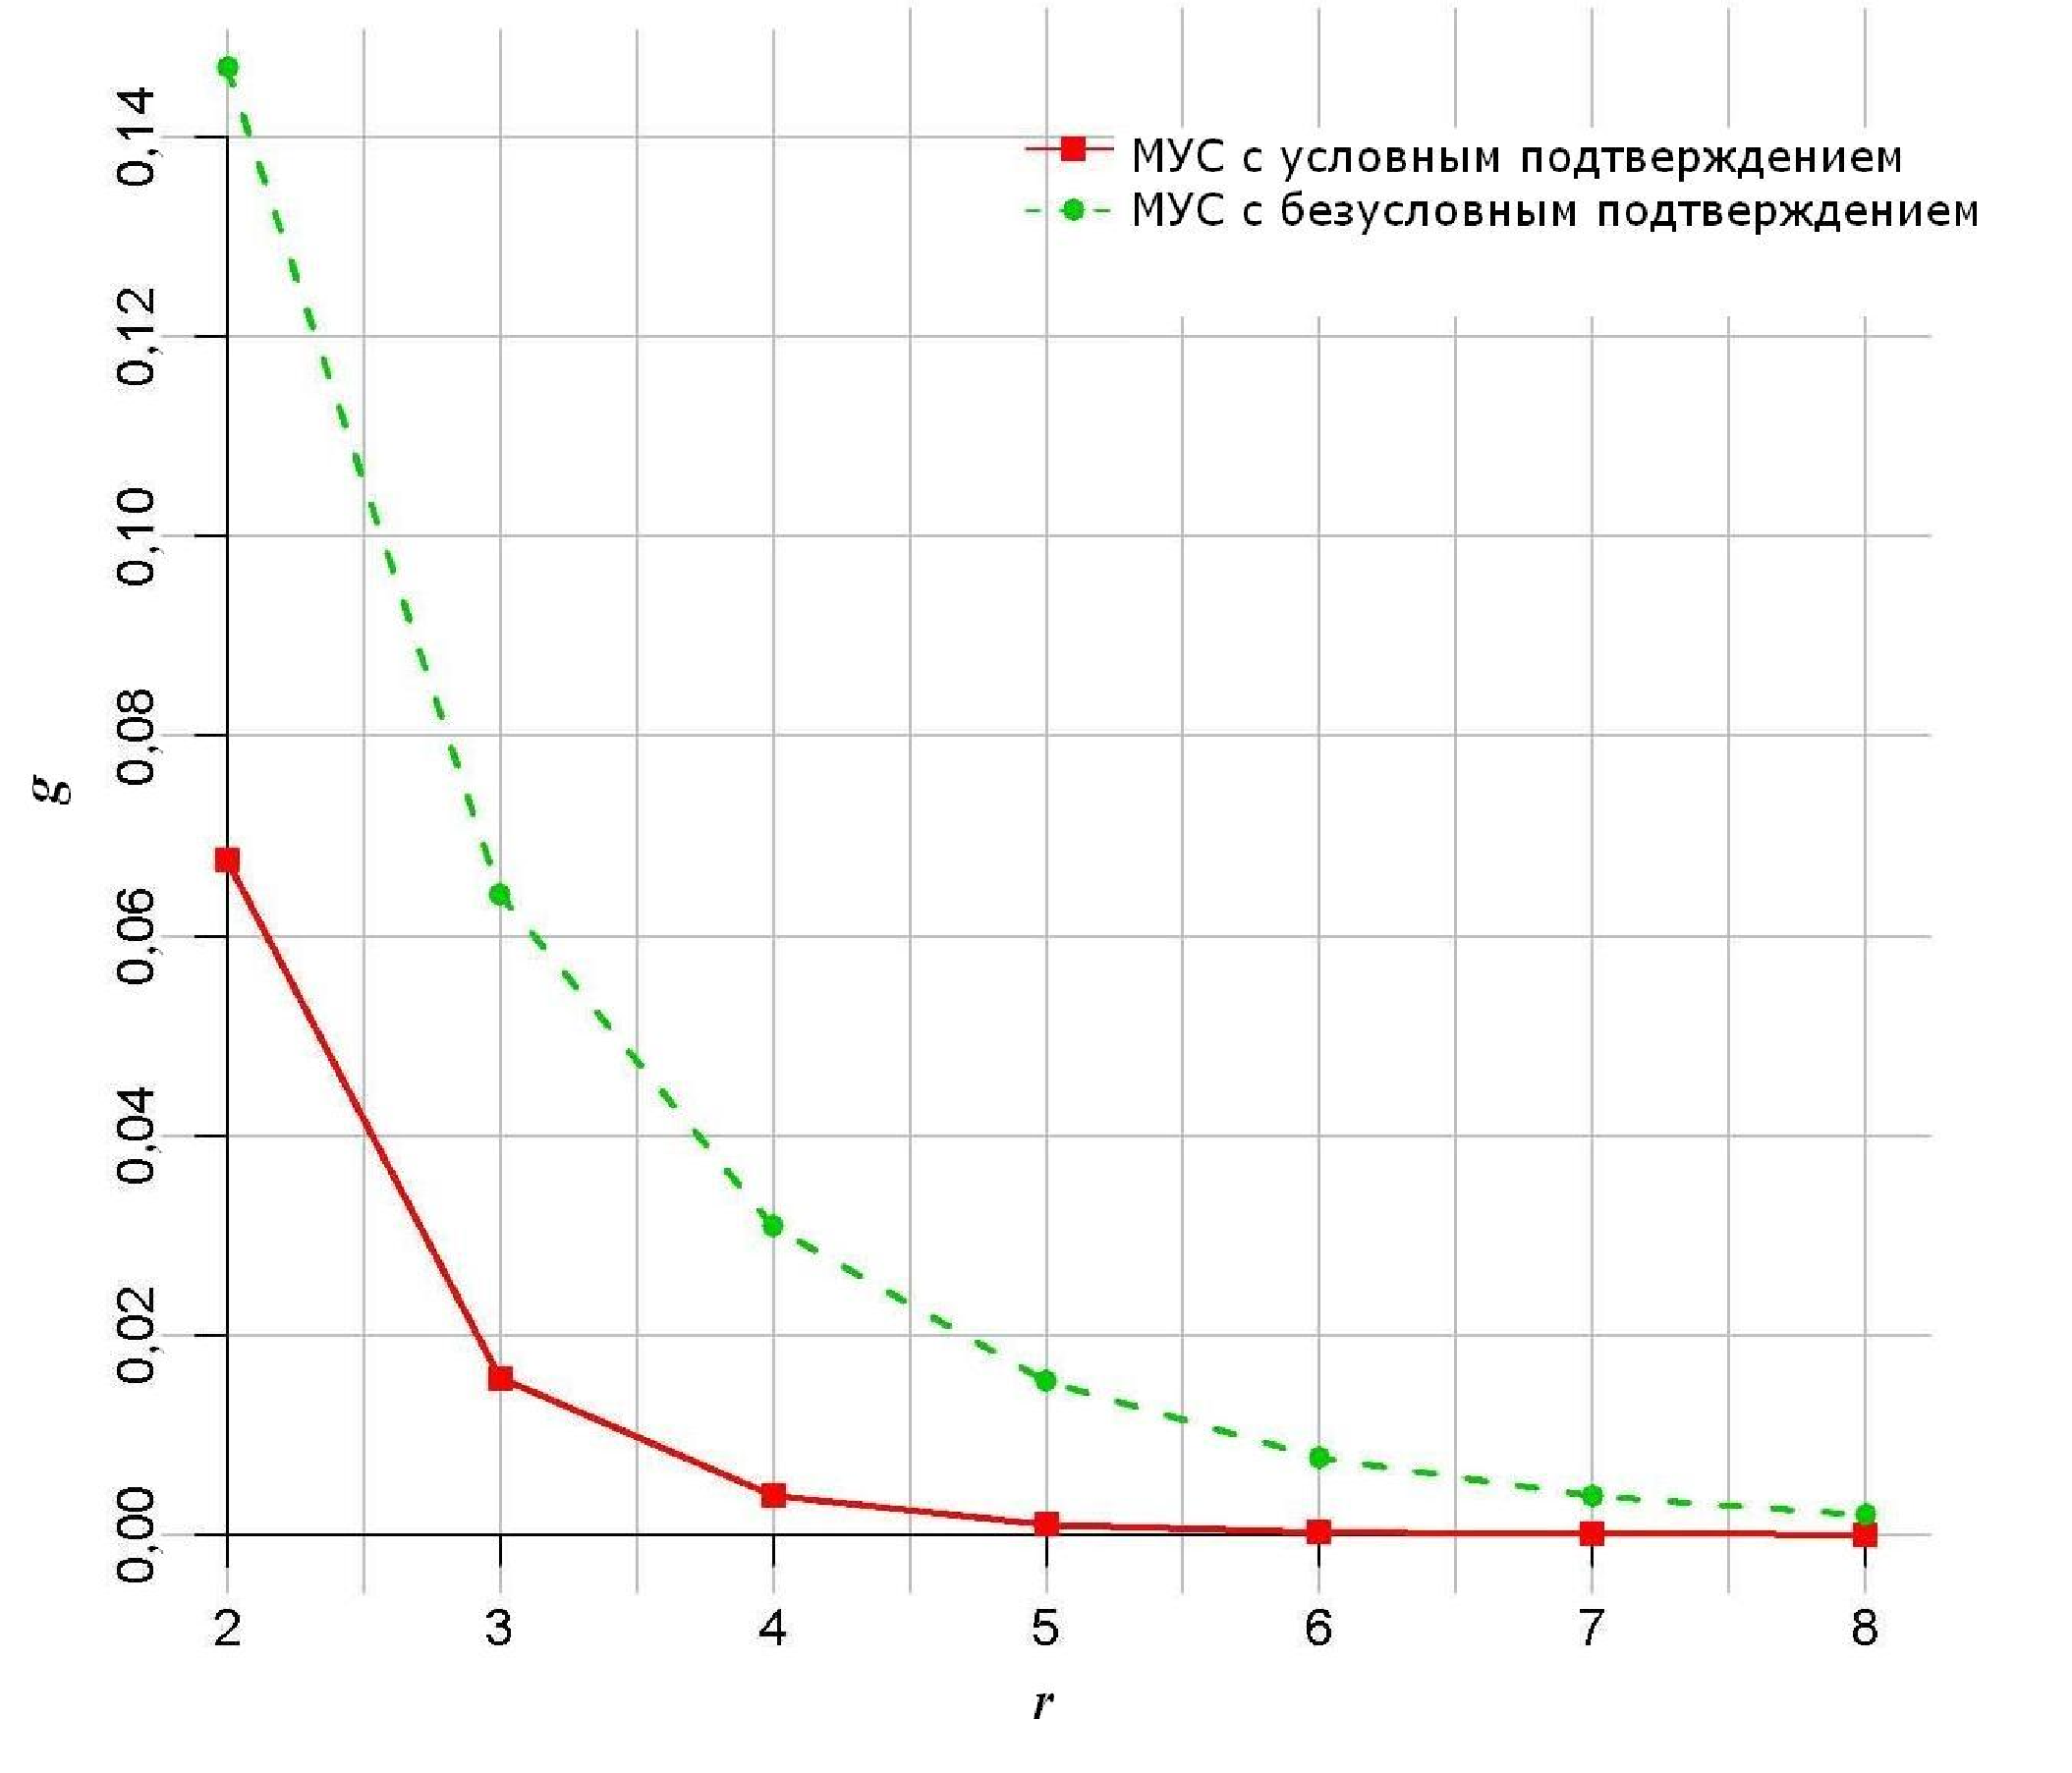
\includegraphics[width=0.86\textwidth]{pic/ParetoRjpg.pdf}
%\end{center}
%\caption{\label{pic:paretoR} Кривые эффективности МУС с условным подтверждением и МУС с безусловным подтверждением}
%\end{figure}
%
%
%
%Согласно (\ref{eq:task:g}) $g' = \frac{1}{2 \cdot 40} \approx 0.025$. Видно, что максимум $g$ достигается в окрестности точки $\pi = \pi_0 = 0.5$, что равносильно $p = p_0$. Тогда ограничению (\ref{eq:task:g-g0}) удовлетворяют значения параметров $r \geq 5, s=r$ для МУС с безусловным подтверждением и  $r \geq 3, s=2r-1, l=r-1$ для МУС с условным подтверждением. Выбирая минимальное значение $r$ согласно (\ref{eq:task:r}), получаем искомые значения параметров $r=5,s=5$ для МУС без подтверждения $r=3,s=5,l=2$ для МУС с подтверждением. Заметим, что уже здесь видно, что МУС с подтверждением позволяет нам выбрать меньшее значение $r$, что согласно (\ref{eq:task:r}) является более эффективным.
%
%Определив множество значений параметров, удовлетворяющих (\ref{eq:task:pi-eq}), выберем те, которые удовлетворяют (\ref{eq:task:g}) и (\ref{eq:task:delta}).
%
%Из оставшихся наборов значений параметров МУС наилучшим будет набор с наименьшим значением $r$, другими словами, удовлетворяющий критерию (\ref{eq:task:Tinfo}).
%Итак, путь $p_0 = 0.5$, $T_0 = 40$. Из таб.~\ref{table:RSpNoConfirm}, \ref{table:RSpConfirm} находим, что условию (\ref{eq:task:pi-eq}) удовлетворяют $r=s$ для МУС без подтверждения и $s=2r-1$ для МУС с подтверждением.


% \input{evaluation}




 %Using (\ref{eq:math:ro-rec}), (\ref{eq:math:P_A}), (\ref{eq:math:P_B}) and averaging $\langle T_{open} (\tau) \rangle$ over $\tau$ we obtain from  (\ref{eq:math:T_open_2}):
%Используя (\ref{eq:math:ro-rec}), (\ref{eq:math:P_A}), (\ref{eq:math:P_B}) и







% \input{appendix}




% \section{Рисунки}


\begin{figure}[!h]
\begin{center}
 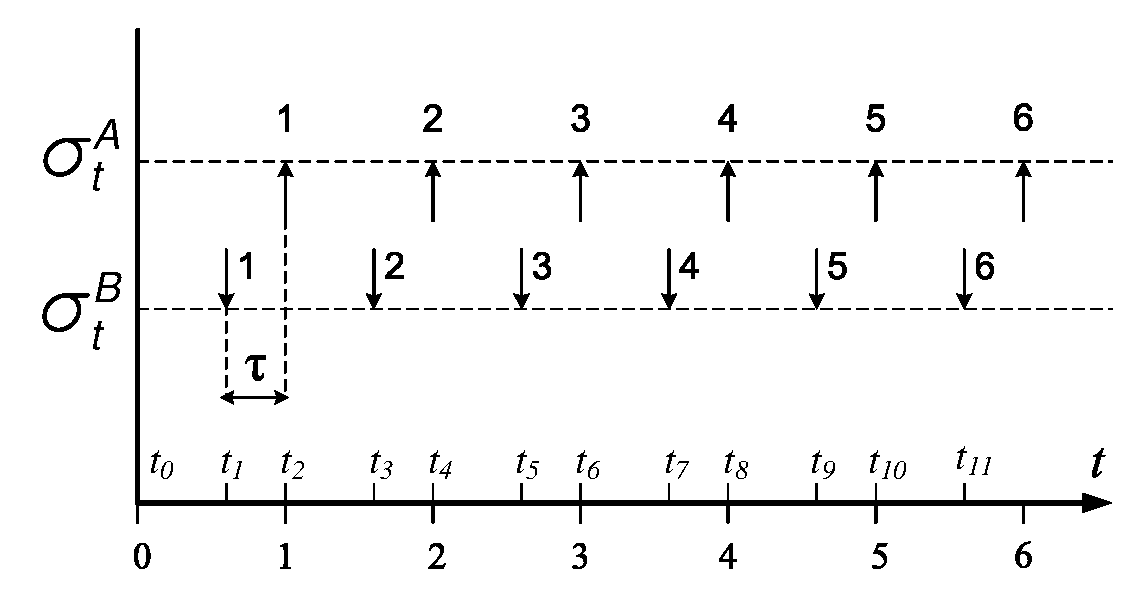
\includegraphics[width=0.5\textwidth]{pic/sigmaABrus.pdf}
\end{center}
\caption{\label{pic:SigmaAB} Последовательности биконов, получаемые станциями $A$ и $B$}
\end{figure}

\begin{figure}[!h]
\begin{center}
\centering
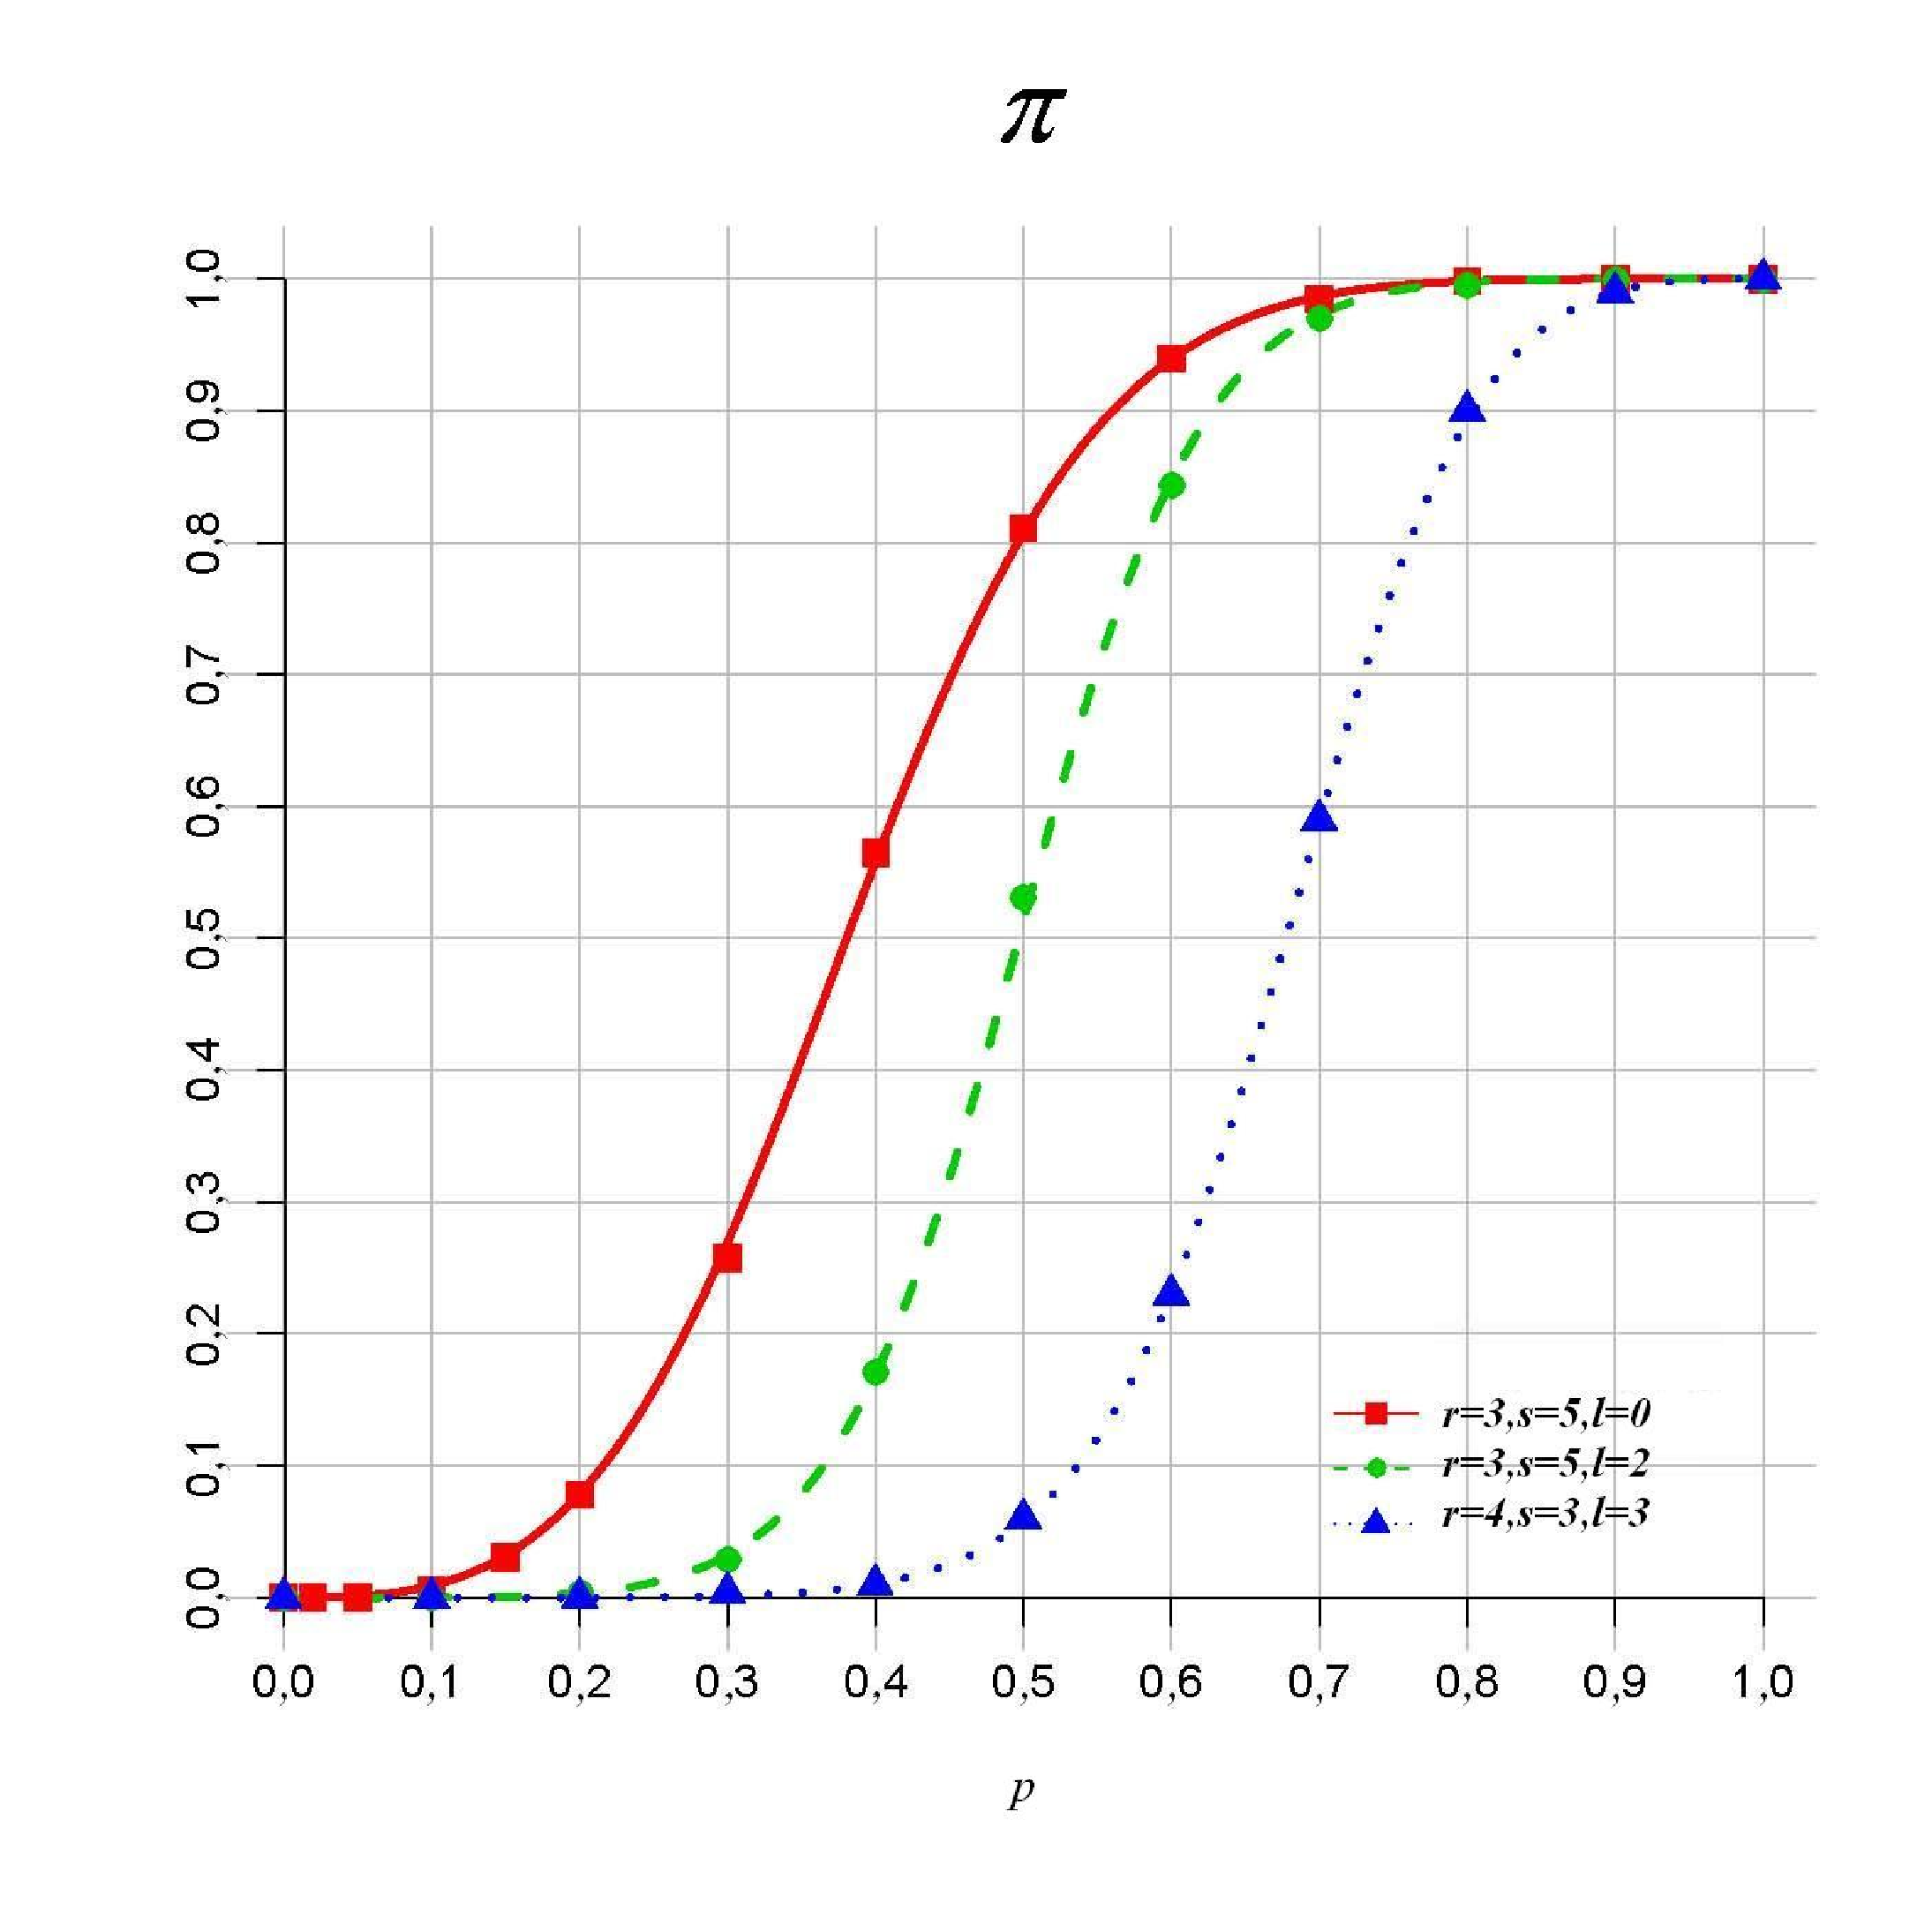
\includegraphics[width=0.5\textwidth]{pic/validation.pdf}
\end{center}
\caption{\label{pic:OpenTimeValidation1} Зависимость $\pi(p)$ для МУС с безусловным ($l=0$) и условным ($l>0$) подтверждением}
\end{figure}

\begin{figure}[!ht]
\begin{center}
\centering
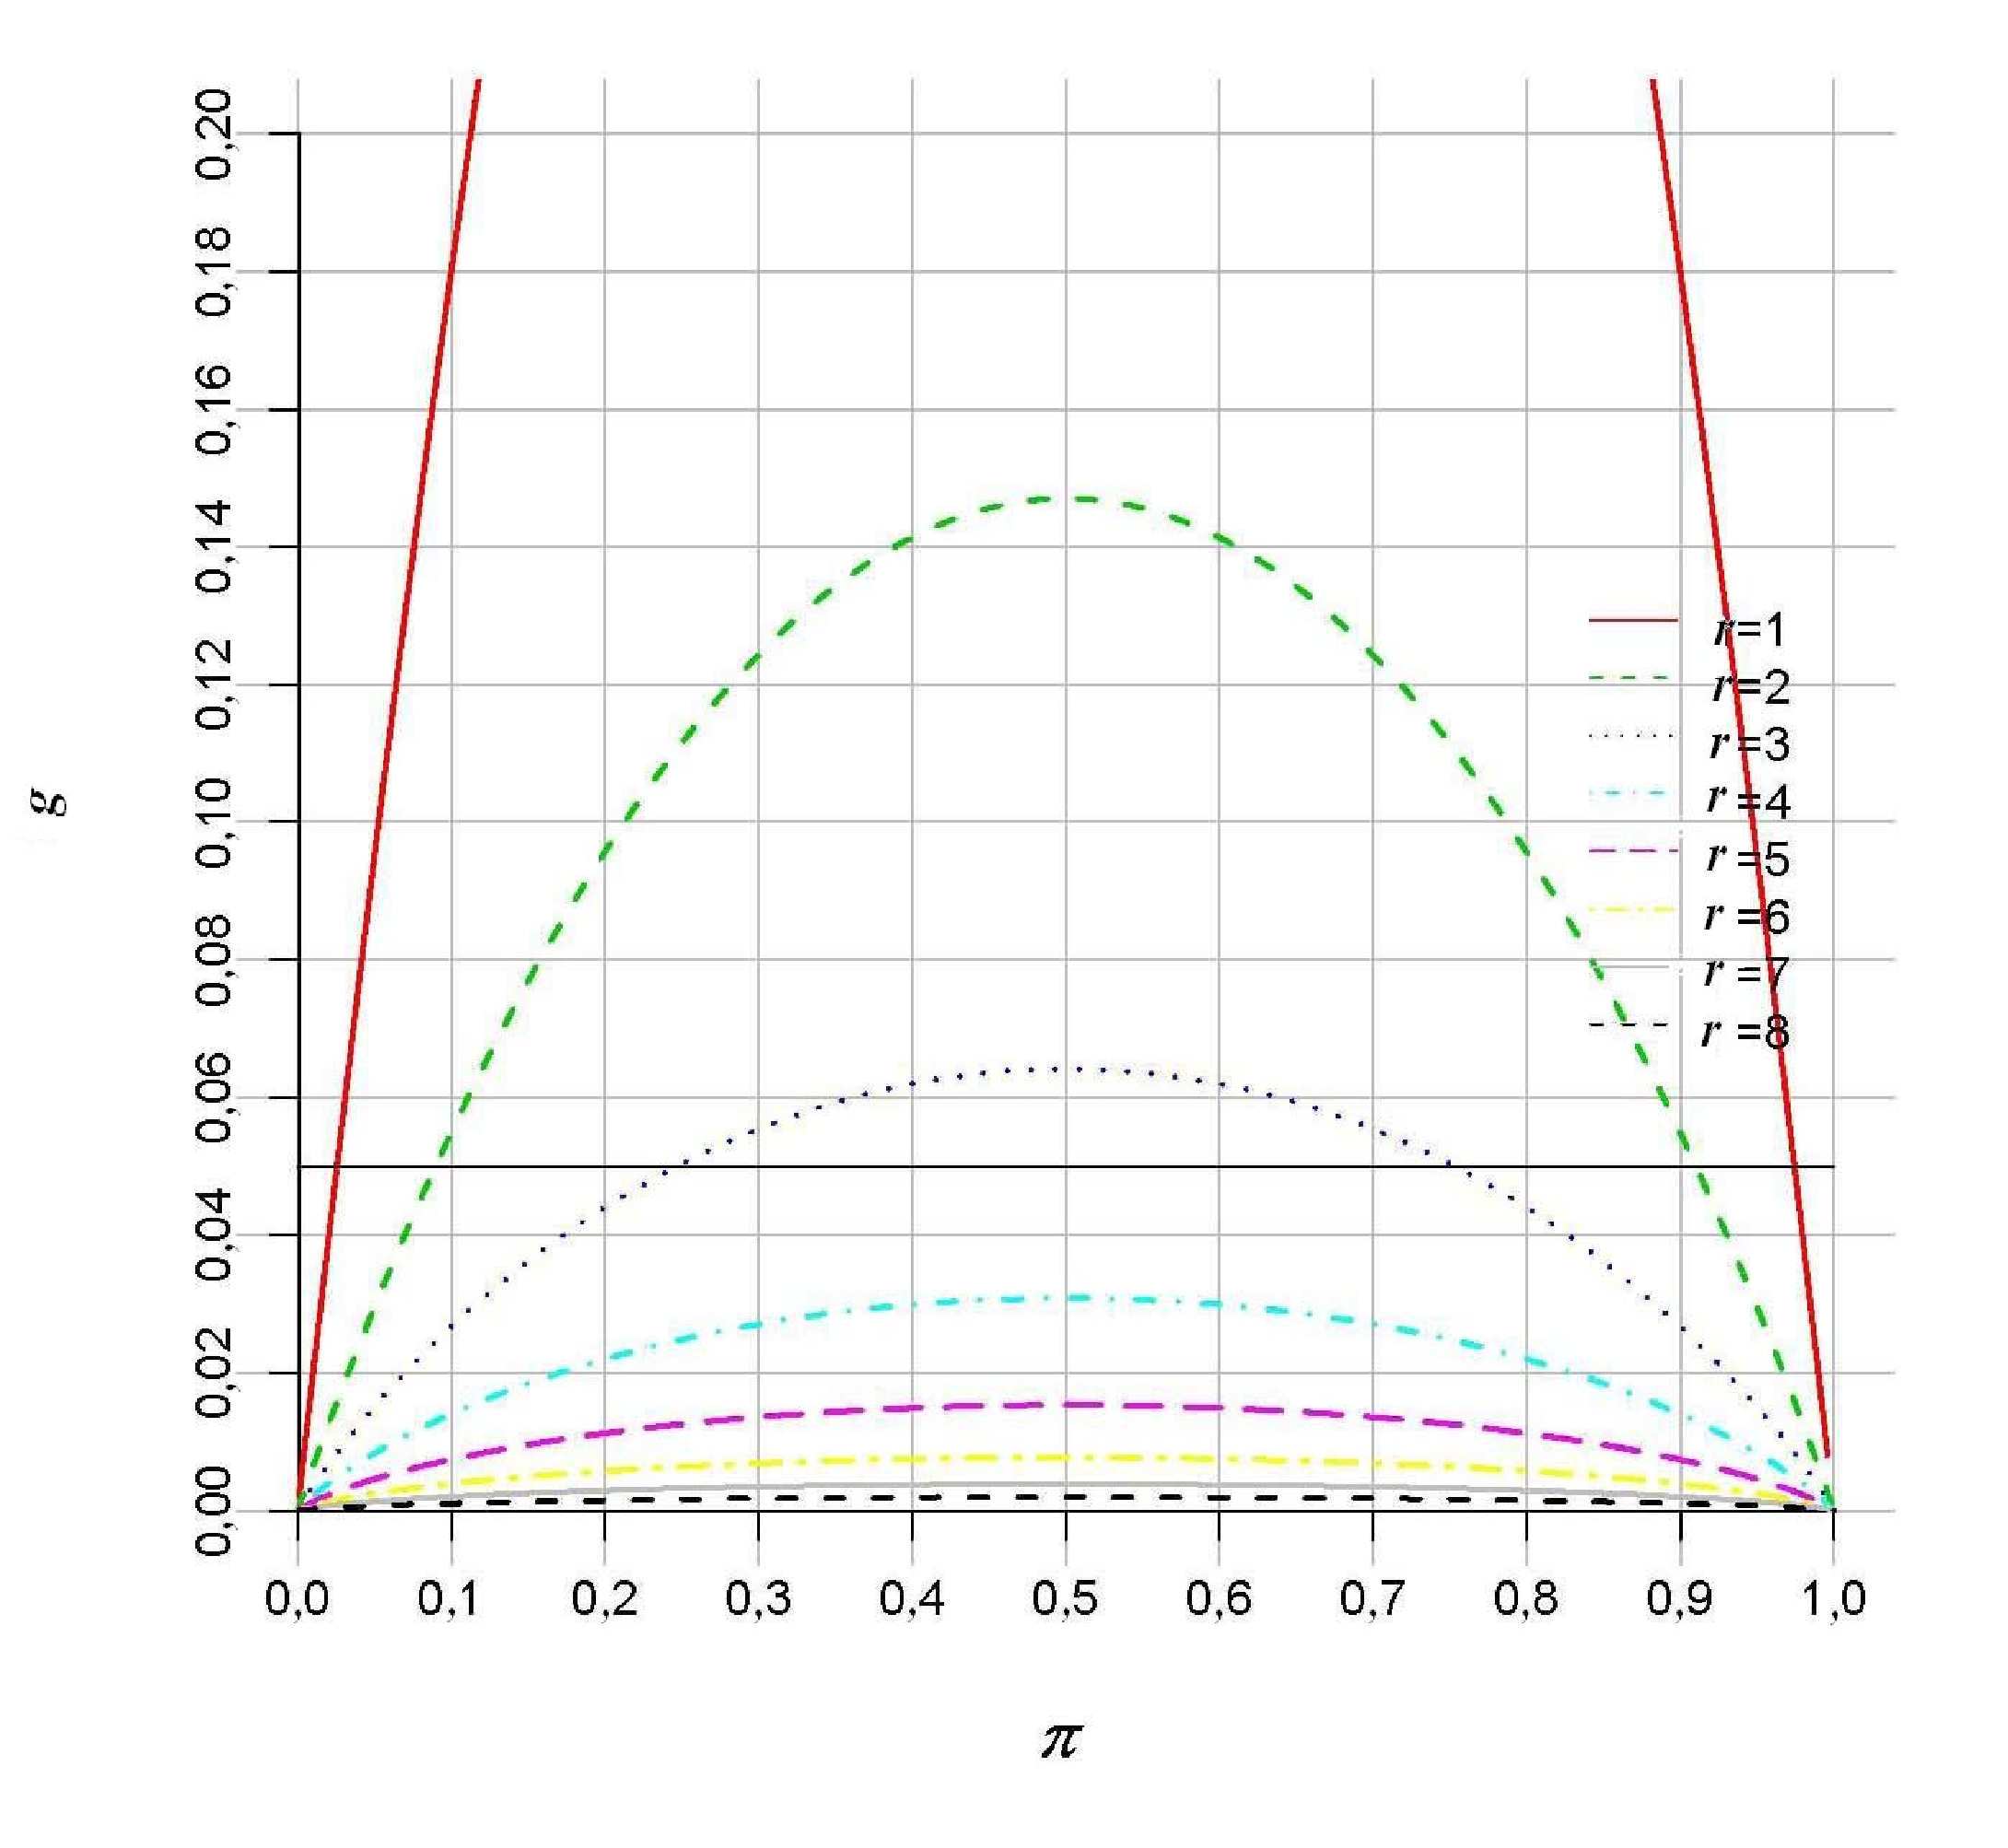
\includegraphics[width=0.5\textwidth]{pic/gFromPiNoConfirm.pdf}
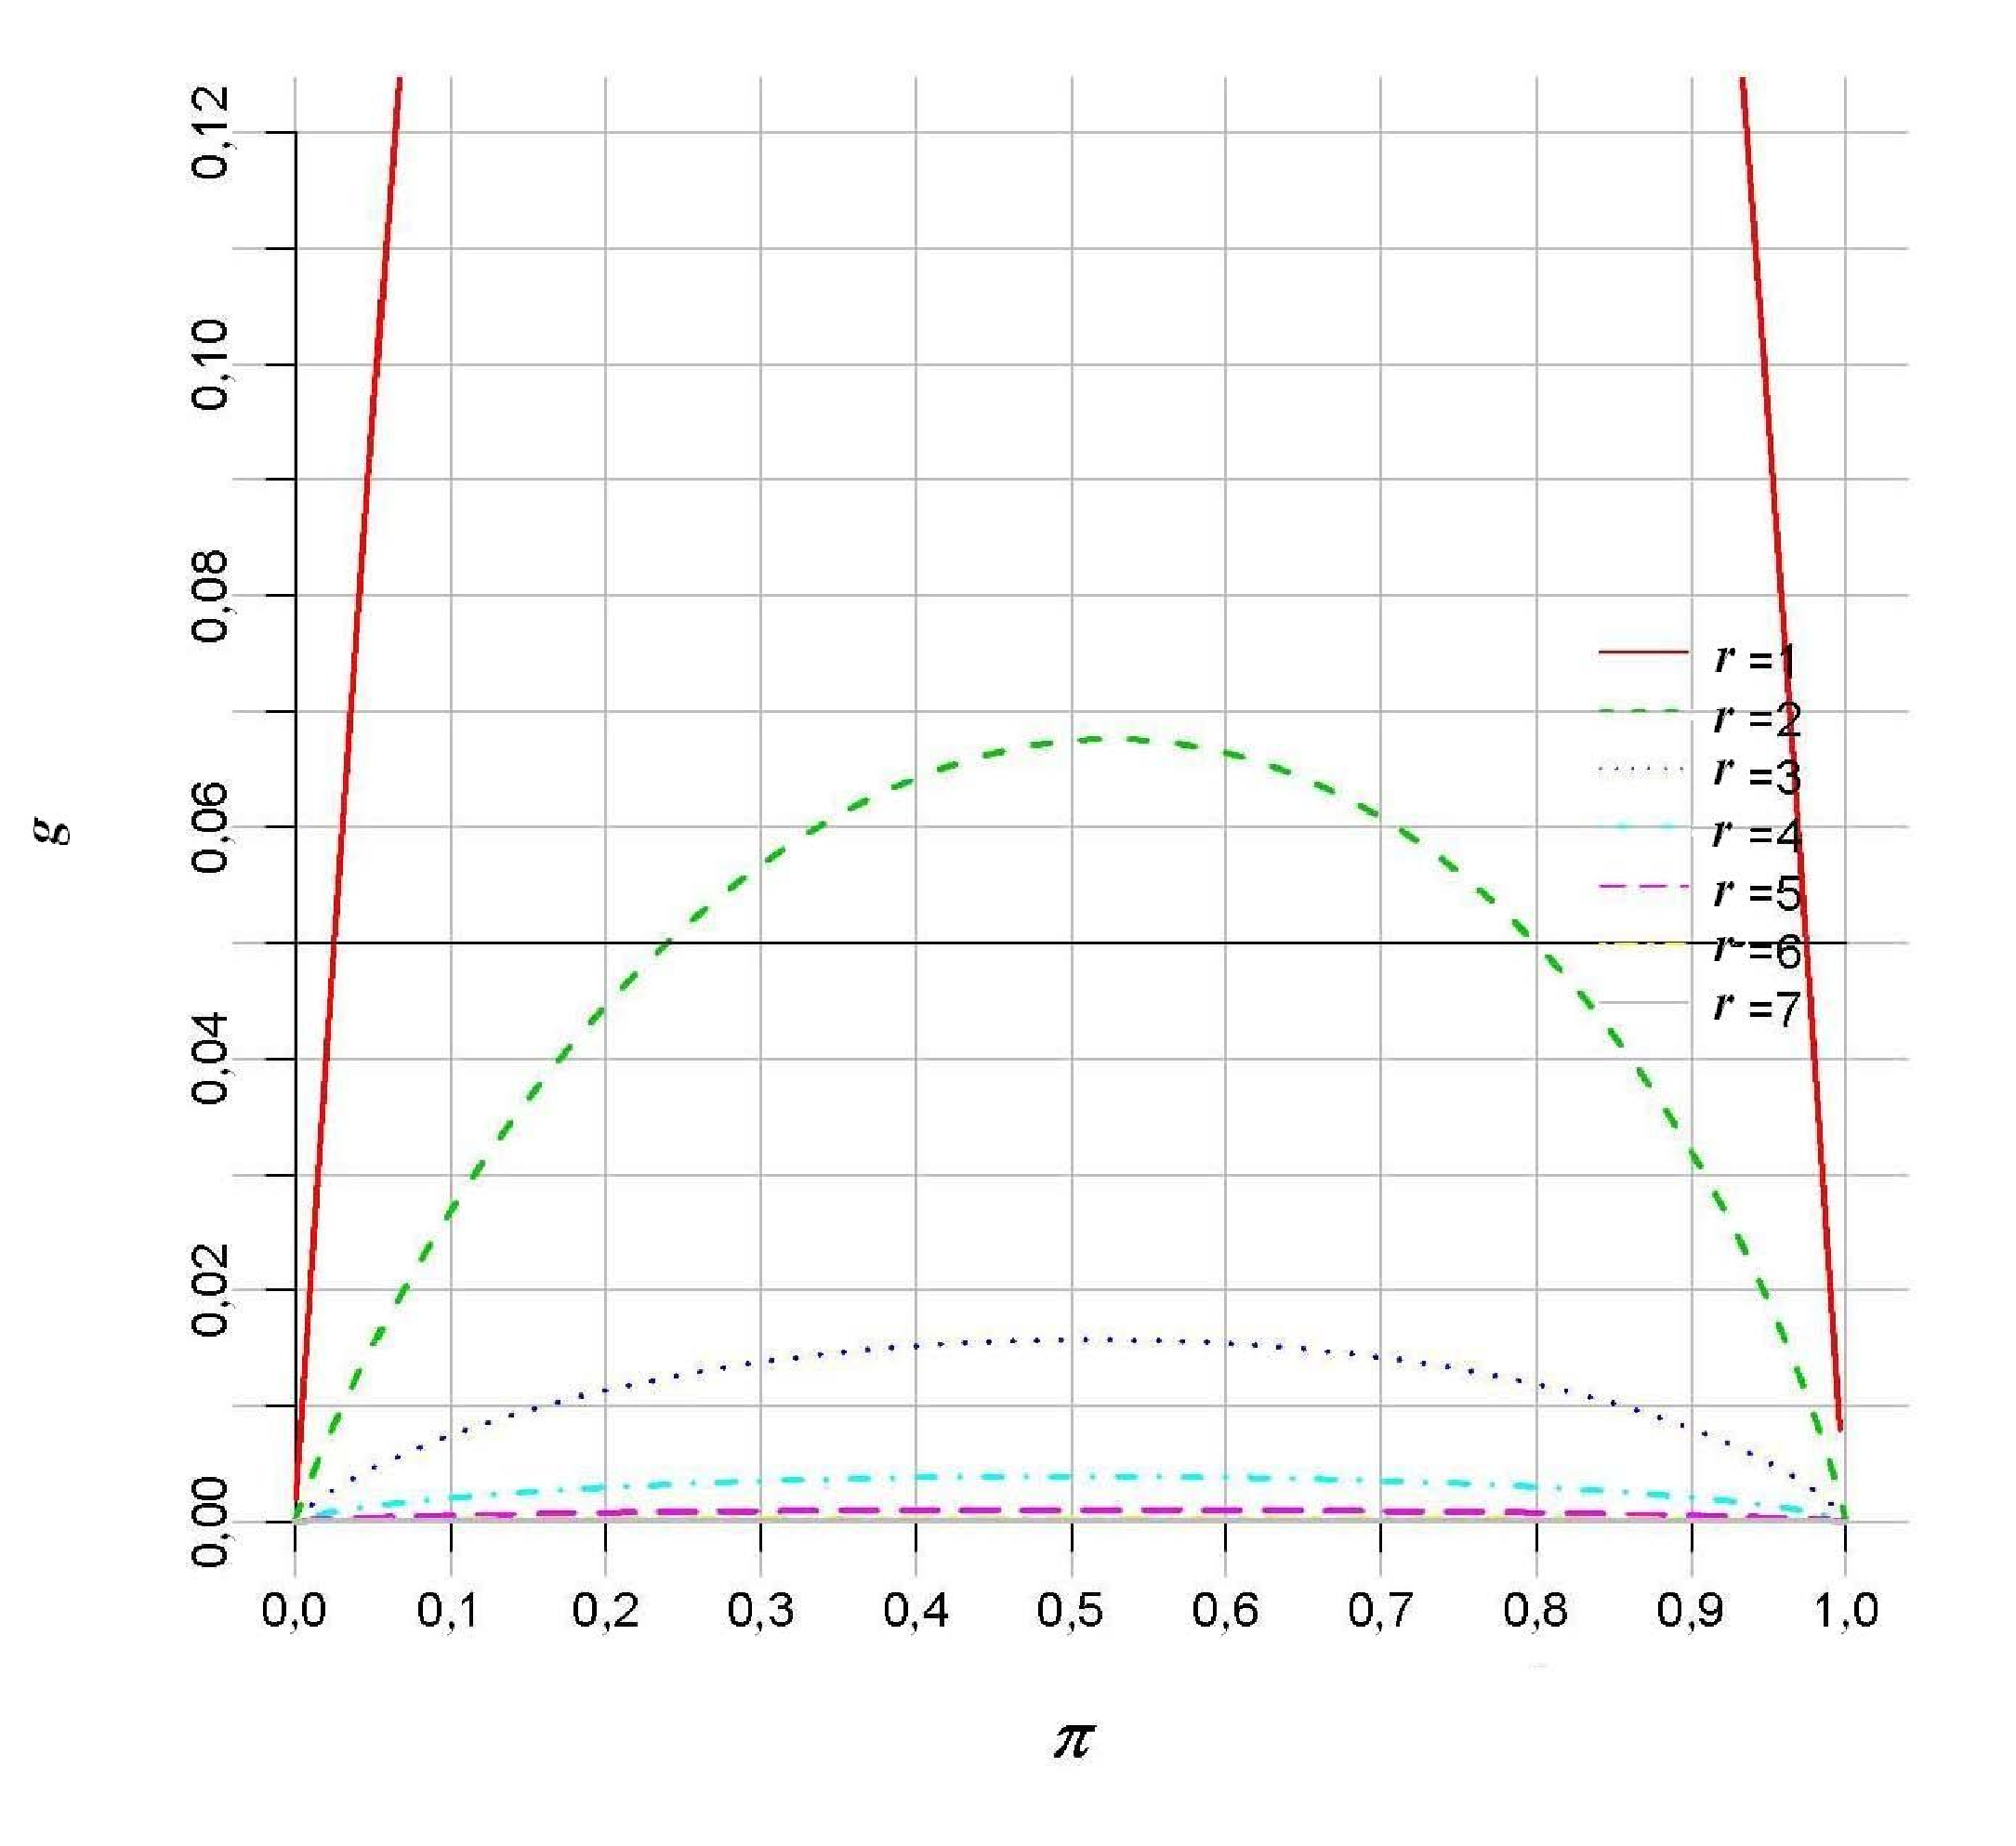
\includegraphics[width=0.5\textwidth]{pic/gFromPiConfirm.pdf}
\end{center}
\caption{\label{pic:g-graph-conf} Зависимости $g(\pi)$: вверху -- для МУС с безусловным подтверждением ($s=r$); внизу -- для МУС с условным подтверждением ($s=2r-1, l=r-1$) при различных $r$}
\end{figure}

\begin{figure}[!htbp]
\begin{center}
\centering
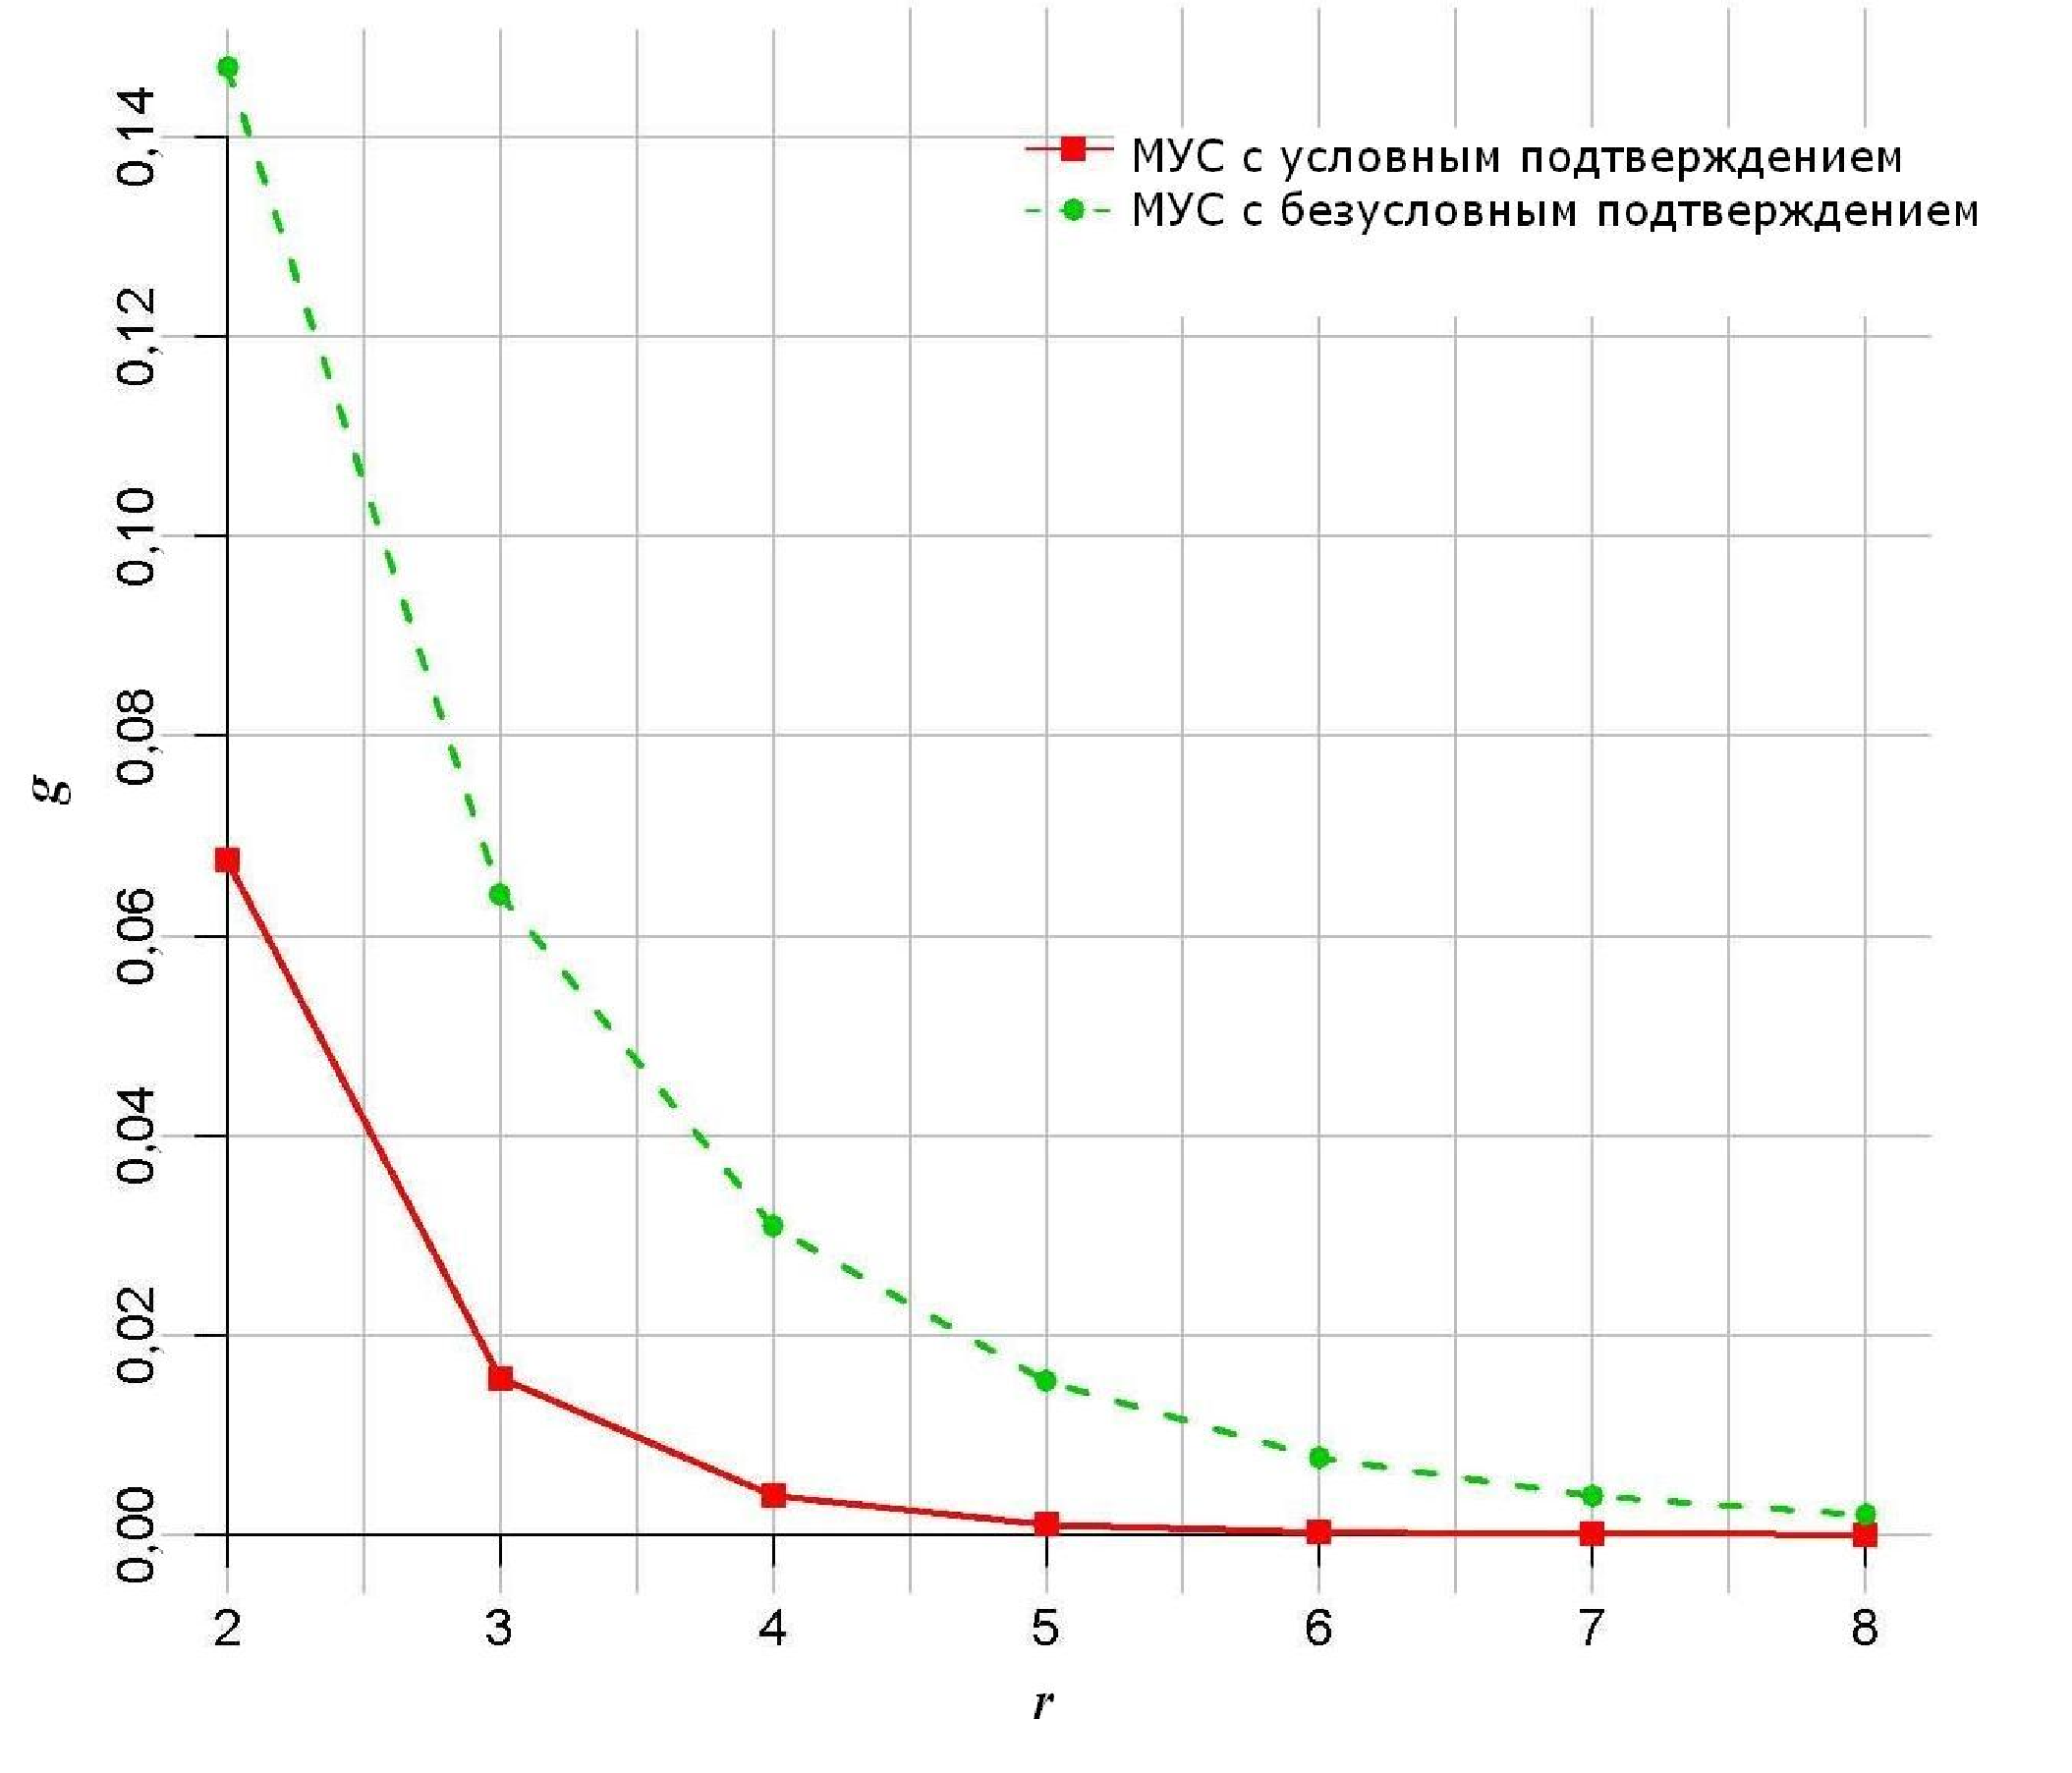
\includegraphics[width=0.5\textwidth]{pic/ParetoRjpg.pdf}
\end{center}
\caption{\label{pic:paretoR} Зависимости $g(r)$ для МУС с условным и безусловным подтверждением}
\end{figure}



% \section{Таблицы}

\begin{table}[!h]
\centering
\begin{tabular}{|c|c|c|c|c|c|c|c|c|c|c|}
\hline
 $s \setminus  r$	&1&	2&	3&	4&	5&	6&	7&	8 \\ %&	9&	10	\\
\hline
  1			&0,5	&0,75	&0,84	&0,88	&0,91	&0,93	&0,94	&0,94 \\ %	&0,959	&0,96	\\
  2			&0,26	&0,5	&0,62	&0,69	&0,73	&0,76	&0,78	&0,8 \\ %	&0,82	&0,83	\\
  3			&0,17	&0,39	&0,5	&0,58	&0,62	&0,66	&0,69	&0,71 \\ %	&0,73	&0,75	\\
  4			&0,13	&0,32	&0,43	&0,5	&0,56	&0,59	&0,62	&0,65 \\ %	&0,67	&0,69	\\
  5			&0,1	&0,28	&0,39	&0,45	&0,5	&0,54	&0,58	&0,6 \\ %	&0,62	&0,64	\\
  6			&0,09	&0,25	&0,35	&0,42	&0,47	&0,5	&0,54	&0,56 \\ %	&0,59	&0,61	\\
  7			&0,07	&0,23	&0,32	&0,39	&0,43	&0,47	&0,5	&0,53 \\ %	&0,55	&0,57	\\
  8			&0,07	&0,21	&0,3	&0,36	&0,41	&0,45	&0,48	&0,5 \\ %	&0,53	&0,55	\\
%  9			&0,06	&0,19	&0,28	&0,34	&0,39	&0,42	&0,46	&0,48	&0,5	&0,53	\\
%  10			&0,05	&0,18	&0,26	&0,32	&0,37	&0,4	&0,44	&0,46	&0,48	&0,5	\\
\hline
\end{tabular}
 \caption{\label{table:RSpNoConfirm} Значения $p_0$ для различных $r$ и $s$ при $l=0$ (МУС с безусловным подтверждением)}
\end{table}

\begin{table}[!h]
\centering
\begin{tabular}{|c|c|c|c|c|c|c|c|c|c|c|}
\hline
$s \setminus  r$	&1&	2&	3&	4&	5&	6&	7&	8 \\ % &	9&	10	\\
\hline
1	&0,5	&0,8	&0,88	&0,91	&0,93	&0,94	&0,95	&0,96 \\ % 	&0,97	&0,97	\\
2	&0,26	&0,6	&0,71	&0,77	&0,81	&0,83	&0,85	&0,87 \\ % 	&0,88	&0,89	\\
3	&0,17	&0,49	&0,62	&0,68	&0,73	&0,76	&0,78	&0,8 \\ %	&0,82	&0,83	\\
4	&0,13	&0,43	&0,55	&0,62	&0,67	&0,7	&0,73	&0,75 \\ %	&0,77	&0,78	\\
5	&0,1	&0,38	&0,5	&0,57	&0,62	&0,66	&0,69	&0,71 \\ %	&0,73	&0,75	\\
6	&0,09	&0,35	&0,46	&0,54	&0,59	&0,62	&0,65	&0,68 \\ %	&0,7	&0,71	\\
7	&0,07	&0,32	&0,43	&0,5	&0,55	&0,59	&0,62	&0,65 \\ %	&0,67	&0,69	\\
8	&0,07	&0,3	&0,41	&0,48	&0,53	&0,57	&0,6	&0,62 \\ %	&0,64	&0,66	\\
%9	&0,06	&0,28	&0,39	&0,45	&0,5	&0,54	&0,57	&0,6 \\ %	&0,62	&0,64	\\
%10	&0,05	&0,26	&0,37	&0,43	&0,48	&0,52	&0,55	&0,58 \\ %	&0,6	&0,62	\\

\hline
\end{tabular}
 \caption{\label{table:RSpConfirm} Значения $p_0$ для различных $r$ и $s$ при $l=r-1$ (МУС с условным подтверждением)}
\end{table}


